\chapter{Quantifying the Forces that Maintain Prophages in Bacterial Genomes}
%\begin{abstract}
Genome sequencing has revealed that prophages, viral sequences integrated in a bacterial chromosome, are abundant, accounting for as much as 20\% of the bacterial genome.  These sequences
can confer fitness benefits to the bacterial host, but may also instigate cell death through induction.  Several recent investigations have revealed that the distribution of prophage lengths is bimodal, with a clear distinction between small and large prophages. In this chapter we develop a mathematical model of the evolutionary forces affecting the prophage size distribution, and fit this model to three recent data sets.  This approach offers quantitative estimates for the relative rates of lysogeny, induction, mutational degradation and selection acting on a wide class of prophage sequences. The model predicts that large prophages are predominantly maintained by the introduction of new prophage sequences through lysogeny, whereas shorter prophages can be enriched when they no longer encode the genes necessary for induction, but still offer selective benefits to their hosts.  
%\end{abstract}

\section{Introduction}
Bacteriophages (phages), the viral predators of bacteria, are the most abundant microorganisms in the biosphere \citep{clokie_phages_2011} and have been critical players in the evolutionary history of bacteria \citep{stern_phage-host_2011}. Many phages reproduce exclusively through the lytic life cycle: after attachment to a bacterial cell surface, the phage infects the bacterium, uses bacterial machinery to produce progeny virions, and then kills the cell, through lysis, to release these viral particles into the environment.  In contrast, temperate phages are defined by their ability to switch between the lytic and lysogenic life cycles.  In the lysogenic life cycle, after infecting the bacterial cell, the phage DNA is integrated into the bacterial chromosome, and does not produce progeny virions \citep{howard-varona_lysogeny_2017}. Prophage refers to phage DNA which has been integrated into the bacterial chromosome in this way, and bacterial host cells containing prophages are referred to as lysogens \citep{weinbauer_ecology_2004}. Prophage sequences are then transmitted vertically with the host bacterial genome as the host cell divides into daughter cells.  

Prophages are frequently identified in sequenced bacterial genomes and contribute up to  20\%  of a bacterial DNA sequence \citep{casjens_prophages_2003}. The number of prophages in a bacterial genome is extremely variable, ranging from zero to more than a dozen prophages per genome \citep{touchon_genetic_2016}. The identity of these prophages also varies both within and among species \citep{mottawea_salmonella_2018}, with prophage content being particularly high in bacterial pathogenic strains \citep{canchaya_impact_2004}.

While integrated in the bacterial genome, many temperate virus genes are not expressed and are thus not under selection for function \citep{lawrence_where_2001}. Prophages are thus subject to loss-of-function mutations or deletions \citep{casjens_prophages_2003} which are hidden from purifying selection.  This sequence degradation may affect genes required for lysis and may render the prophage defective, that is, unable to enter the lytic life cycle.  Defective or ``cryptic'' prophages are abundant in bacterial genomes, for example  \textit{Escherichia coli} K-12 contains nine cryptic prophage elements \citep{wang_cryptic_2010}. Some defective prophages are able to re-enter lysis with the help of co-infecting phages \citep{matos_enterococcus_2013}.

Recently, using \textit{PhiSpy}, a bioinformatics tool for identifying prophages \citep{akhter_phispy:_2012}, $36,488$ prophages  were identified from the analysis of over $11,000$ bacterial genomes; $83 \%$ of the bacterial genomes contained at least one prophage \citep{kang_prophage_2017}. In a similar study \citep{costa_genomic_2018}, $4,122 $ prophages were identified in $795$ genomes of  \textit{Acinetobacter baumannii}, for an average of 5 prophages per bacterial genome; PHAge Search Tool (PHAST) \citep{zhou_phast:_2011} was used for the identification of these prophages. 
Of these prophages,  $78\%$  were identified as defective  \citep{costa_genomic_2018}. Using PHASTER (PHAge Search Tool - Enhanced Release) \citep{arndt_phaster:_2016}, $11,297$ prophages were identified in $1,760$ \textit{Salmonella enterica} genomes, for an average of $6.4$ prophages per bacterial genome \citep{mottawea_salmonella_2018}. Due to this abundance of lysogeny in the bacterial world, it has been suggested that for temperate phages, the amount of viral genetic material encoded in  prophages likely surpasses the total amount of viral DNA in free phage particles \citep{wahl_prophage_2017}. 
 
The relationship between bacteria and prophage is complex and multifaceted. Integration of the phage genome into a bacterial genome may be a survival strategy for the phage \citep{refardt_tuning_2010}, at the risk of abandoning an independent, predatory existence. The acquisition of viral genomes comes with obvious costs for the bacterial host cell, most importantly the risk
of future lysis \citep{ptashne_genetic_2004}, as well as the energy costs of maintaining extra genetic material in the bacterial genome \citep{millan_interactions_2015}. But prophage often carry beneficial genes and may confer novel adaptive traits to their bacterial hosts, which in turn helps the prophages themselves to proliferate \citep{bobay_pervasive_2014}.  

Table \ref{table:bt} lists several such benefits, conferred by prophages to their bacterial hosts. These traits are often interrelated, for example, prophages can enhance the host's capacity to form biofilm and biofilm can enhance antibiotic resistance. Biofilm bacteria are $500 - 1000$ times more resistant to antibiotics as compared to planktonic  (free-living) bacteria \citep{harper_bacteriophages_2014}. 
    \begin{table}[t]
\centering
\begin{tabular}{p{7.8cm}p{7cm}}
\hline
Beneficial trait & Reference \\
\hline
protection from infection by the same phage (super infection exclusion) & \cite{canchaya_impact_2004,hofer_superinfection_1995}\\

protection from phagocytosis & \cite{meltz_steinberg_grazing_2007} \\

increase in cell growth rate & \cite{wang_cryptic_2010} \\

increase in antibiotic resistance & \cite{haaber_bacterial_2016, wang_cryptic_2010} \\

increase in tolerance to environmental stress & \cite{edlin_reproductive_1977, wang_cryptic_2010}\\

enhanced ability to form biofilm & \cite{wang_cryptic_2010, godeke_phage-induced_2011}\\
virulence factors & \cite{hacker_ecological_2001,fortier_importance_2013, banks_fundamental_2002}\\
 
suppression of metabolic activity
to increase survival in harsh environments & \cite{paul_prophages_2008}\\

activation/deactivation of regulatory switches   & \cite{feiner_new_2015}\\
 
adaptation to new host & \cite{diene_prophages_2017}\\
\hline
\end{tabular}
\caption{Beneficial traits that bacterial hosts may acquire from integrated prophages. }
\label{table:bt}
\end{table}
 
 Although prophages are quite stable within bacterial genomes, intact prophages are able to initiate the lytic life cycle.
 Induction results in the death of the bacterial host cell and release of progeny virions. Some prophages, like $\lambda,$ excise from the bacterial chromosome to initiate the lytic life cycle, while for others, like Mu, the original prophage sequence remains in the bacterial host genome while viral particles are produced \citep{shapiro_molecular_1979}. Induction can be triggered spontaneously \citep {fothergill_effect_2011, james_differential_2012} or by DNA damaging agents, including external stimuli such as exposure to UV light or antibiotics \citep {barnhart_prophage_1976, lopez_induction_2014}. 

 Prophage sequences are the single most prominent 
 source of genetic diversity within bacterial populations \citep{fortier_importance_2013}, and  prophage-encoded genes contribute to many aspects of bacterial physiology. The contribution of prophages to bacterial virulence, as well as to antibiotic resistance, have been particularly well-studied \citep{wagner_bacteriophage_2002,fortier_importance_2013, haaber_bacterial_2016}. 
Understanding the spread and maintenance of prophage sequences in bacterial genomes is thus an important first step in estimating the impact of phage populations on these critical public health issues.  Our aim is to make use of the wealth of recent data
 regarding the distribution of prophages in bacterial genomes to shed light on the evolutionary forces responsible for maintaining prophage sequences.  We seek answers to basic questions about prophage evolution, such as: how does the rate at which prophage enter bacterial genomes through lysogeny compare with the induction rate; how does loss through induction compare with loss through mutational degradation; can we quantify the magnitude of the selective benefit conferred by prophages to their hosts?

\subsection{The prophage size distribution} \label{psd}
 When a prophage is first integrated into a bacterial genome, its length is determined by the sequence length of the corresponding viral genome. 
 Random mutation in the bacterial genome, however, is strongly biased toward deletions \citep{kuo_deletional_2009,mira_deletional_2001, danneels_patterns_2018}.  In addition, intact prophages may be lethal to the host cell, thus there should be strong selection for inactivation. Hence in a random sample of prophage sequences, one might expect a few large prophages, corresponding to fully inducible sequences, followed by a gradient of smaller and smaller prophages that have been subject to degradation over evolutionary timescales \citep{bobay_pervasive_2014}. In other words, assuming prophage sequences enter bacterial genomes at a relatively constant rate, we might expect a unimodal distribution with a peak on the right and a long tail to the left (negative skewness).
 
 In contrast with this expectation, three recent datasets -- available in public databases and discussed in greater detail below -- suggest that the distribution of prophage lengths, across a wide variety of bacterial species, is multimodal
 \citep{bobay_pervasive_2014,crispim_screening_2018,brueggemann_pneumococcal_2017,leplae_aclame:_2010}.  In the sections to follow, we will use each of these datasets to determine the simplest evolutionary model that is consistent with these data;  in other words, which forces or processes are, at a minimum, necessary to recover these distributions?
 
 The data sets we analyze further are:
 
 \textbf{Data Set 1} \citep{bobay_pervasive_2014}: Bobay et al. identified $624$ prophages  (474 from \textit{E.~coli} and 150 from \textit{S.~enterica}) and recovered a bimodal distribution of prophage lengths; see Figure~ 1A. Note that prophages that had no resemblance to core phage genomes from this study were discarded.
 
\textbf{Data Set 2} \citep{crispim_screening_2018}: $128$ prophages in \textit{Desulfovibrio}, the sulphate-reducing bacteria,  were  shown to have a bimodal or possibly trimodal distribution; see Figure~1B.

\textbf{Data Set 3} \citep{leplae_aclame:_2010}: The ACLAME database (\href{http://aclame.ulb.ac.be}{http://aclame.ulb.ac.be}) contains $760$ prophage sequences. These data were retrieved using Prophinder \citep{lima-mendez_prophinder:_2008}, a prophage detection algorithm. Note that this data set includes a sparse tail of prophages with a length greater than 60 kb; in the data fitting described below, we neglect these outliers, reducing the data set from 760 to 737 prophages; see Figure~1C.

A further summary of these data sets is provided in Table \ref{table:2}. 

In addition to these three publicly-available datasets, further evidence regarding the distribution of prophage lengths has recently appeared in  a study of the molecular epidemiology of \textit{Pneumcocci} \citep{brueggemann_pneumococcal_2017}; $482$ prophages were collected from clinical isolates that spanned 36 countries and nearly a century (1916-2008). Although the lengths of individual prophages in these data are not publicly available, overall the lengths exhibit a bimodal distribution, as shown in Figure~1D. 

\begin{figure}[H]
    \centering
    \begin{subfigure}[t]{0.45\textwidth}
    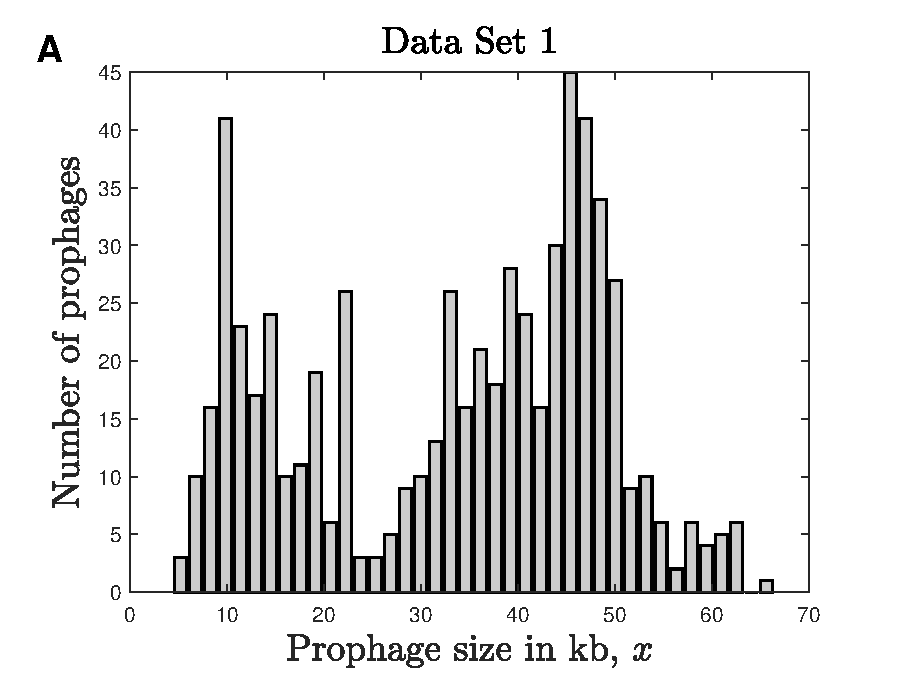
\includegraphics[scale=0.55]{bobbar}
    %\subcaption[subfigcapskip = 50pt]{Data Set 1.}
    %\label{fig:bob_bar}
    \end{subfigure}\hfill
    \begin{subfigure}[t]{0.45\textwidth}
    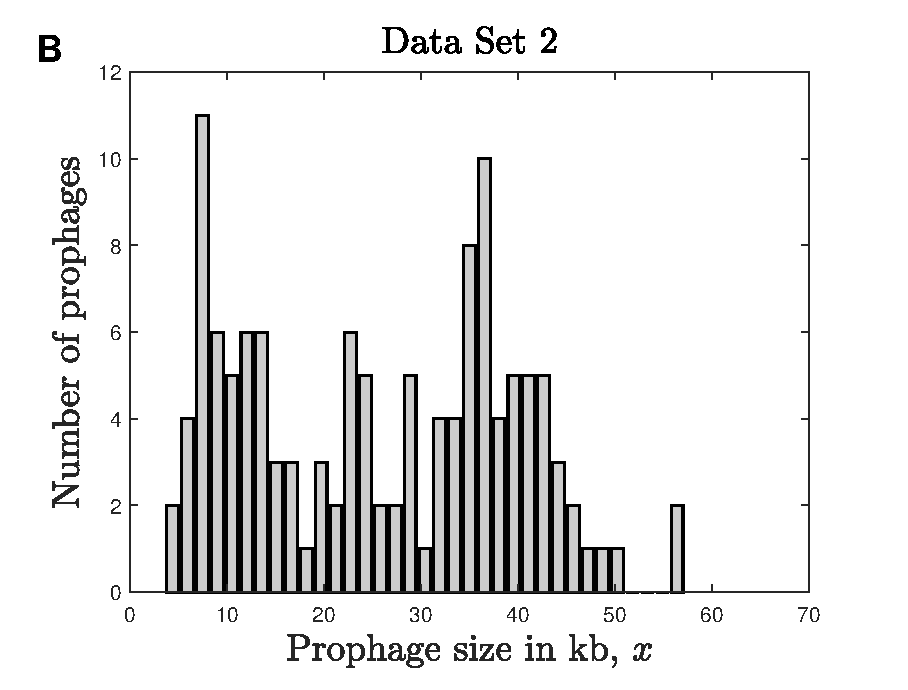
\includegraphics[scale=0.55]{desubar.eps}
       % \subcaption[subfigcapskip = 50pt]{Data Set 2. }
        %\label{fig:desu_bar}
    \end{subfigure}\hfill
    \begin{subfigure}[t]{0.45\textwidth}
    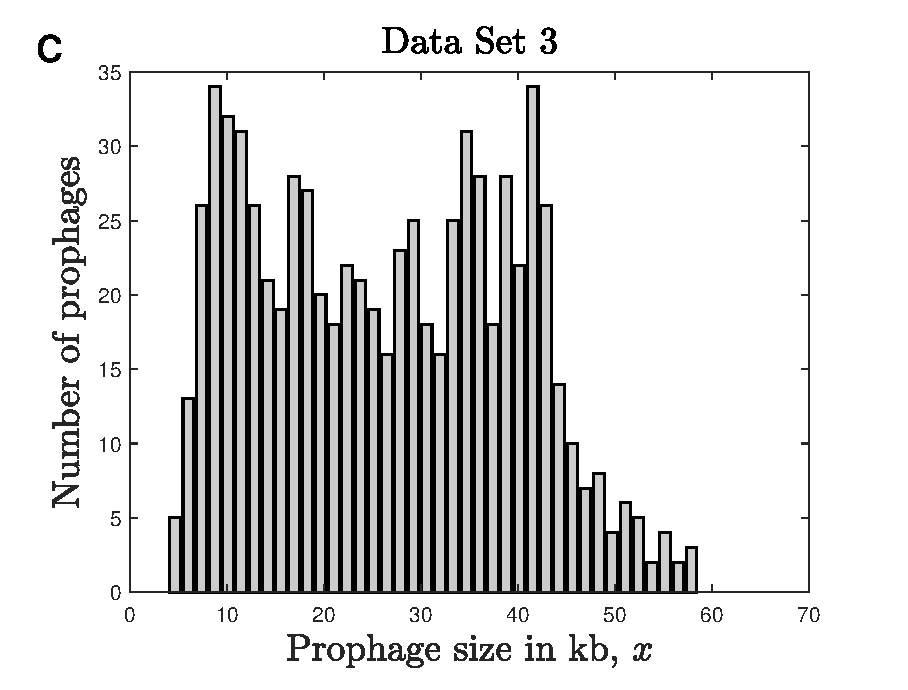
\includegraphics[scale=0.55]{ALCLbar.eps}
            %\subcaption[subfigcapskip = 50pt]{Data Set 3.}
            %\label{fig:ACL_bar}
    \end{subfigure}\hfill
     \begin{subfigure}[t]{0.45\textwidth} 
    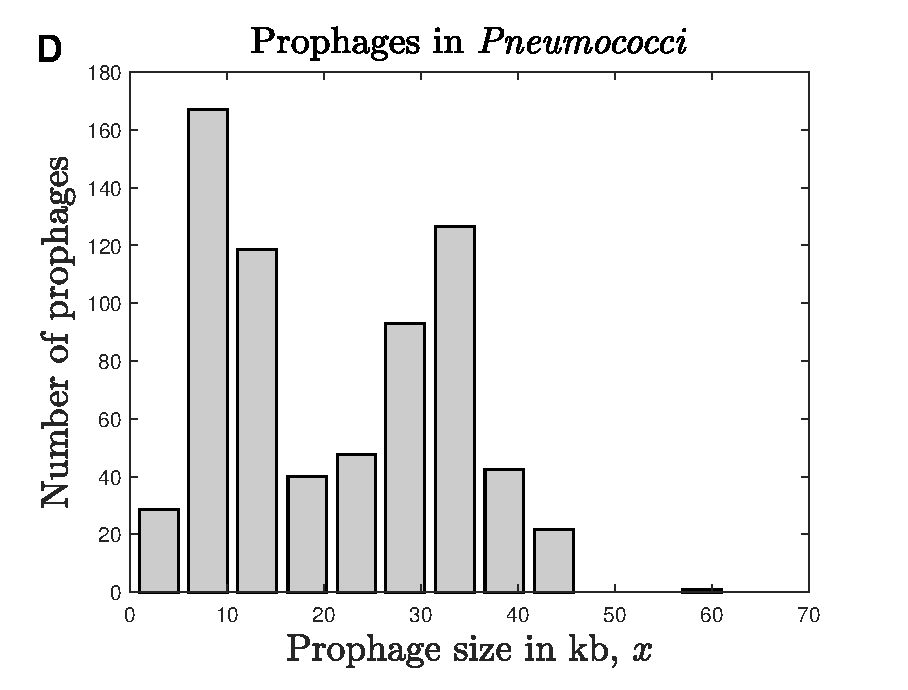
\includegraphics[scale=0.55]{brubar.eps}
    % \subcaption{Prophages in \textit{Pneumococci}.}
     %\label{fig:brug_bar}
     \end{subfigure}\hfill
    \caption[Prophage size distributions.]{ Prophage size distributions.   (A) Prophages identified in \textit{E.~coli} and \textit{S.~enterica} \citep{bobay_pervasive_2014}. (B) Prophages identified in \textit{Desulfovibrio} \citep{crispim_screening_2018}. (C) Prophages across a range of sequenced bacterial genomes \citep{leplae_aclame:_2010}.  (D) Prophages identified in \textit{Pneumococci} \citep{brueggemann_pneumococcal_2017}.}
\label{fig:data}
\end{figure}

%\renewcommand{\baselinestretch}{1.0}
\begin{table}[H]
\centering
\begin{tabular}{ p{1.2cm}p{1.5cm}p{1cm}p{1cm}p{1.5cm}p{3.5cm}p{3.5cm}}
\hline
Data Set & Prophage number & Min (kb)& Max (kb)& Average (kb)& Bacterial Species &Reference \\
\hline
1 & 624 &4.348& 66.345& 33.268 & \textit{E.~coli}, \textit{S.~enterica} &\cite{bobay_pervasive_2014}\\

2& 128 & 3.603 & 57.140 & 25.580 & \textit{Desulfovibrio} &\cite{crispim_screening_2018}\\

3& 737 & 3.918 & 58.560  & 26.450 & Diverse &\cite{leplae_aclame:_2010}\\
\hline
\end{tabular}
\caption{Summary of the three data sets analyzed in this study. }
\label{table:2}
\end{table}
%\renewcommand{\baselinestretch}{2.0}

\subsection{Our approach}
 The natural question that arises is: why are prophage size distriubutions so often bimodal?  In a preliminary investigation, \cite{bobay_pervasive_2014} arrived at the conclusion that the bimodal distribution in their data is neither due to taxonomic biases nor due to large neutral deletions of genetic material. 
 In addition, if there were substantial heterogeneity in the prophage integration rate over evolutionary time, we might expect greater diversity in the multimodal distributions observed across a range of bacterial species; in other words, it seems unlikely that the peak at shorter lengths in four datasets is due to a single historical ``burst" of prophage integration.
 The aim of our study is to investigate these prophage distributions in more detail and, using the available data, determine which evolutionary processes are necessary to explain these observations. 
 
 The organization of this article is as follows: in Section~\ref{mm}, we derive a partial differential equation that models the time evolution of the prophage distribution, including expressions for the effects of mutation, selection, horizontal gene transfer and induction. In Section~\ref{ns}, we describe our analysis of the model, including model selection and fitting the model to the available data sets. In Section~\ref{results}, we present the results of data fitting. Finally, in Section~\ref{discussion}, we discuss the conclusions derived from this analysis and suggest further directions.
  
\section{Model Derivation}\label{mm}
To better understand the observed distributions of prophage lengths, we seek an expression for the expected frequency of prophages of length $x$, $P(x)$, in a population of bacterial genomes.  Here $x$ is prophage length in kb, with $x_{0}<x<x_{M}$ ($x_{0}$ and $x_{M}$ are the minimum and maximum prophage length, respectively). We begin by considering the processes that change the distribution of prophages over time, and then solve for the expected steady state (long-term behavior) of the model. Let $Q(x,t)$ be the frequency of prophages of length $x$ at time $t$. After time step $\delta t$, this distribution may change due to: (1) new temperate viral genomes entering the bacterial genome; (2) horizontal gene transfer (HGT) adding new prophages or partial prophages to the existing prophage pool; (3) mutational degradation reducing prophage lengths; (4) selection promoting the proliferation of the bacterial population, and therefore the prophage population; and (5) induction removing prophages from the population . 

Taking into account these five possible processes,
we arrive at the following partial differential equation describing the time evolution of the prophage size distribution:
\begin{eqnarray}\label{pde}
\frac{\partial Q(x,t)}{\partial t}=\alpha f(x)+\, \beta \, g(x)\, +\frac{\partial}{\partial x}\left[D(x)Q(x,t)\right]+r_{S}\,S(x)\,Q(x,t)-r_{I}\,I(x)\,Q(x,t)\,\,.
\end{eqnarray}  
The five terms on the right describe the influx of new prophage via lysogeny, influx via HGT, mutational degradation, selection, and induction respectively.  
The distribution of interest, $P(x)$, if it exists, is the steady state solution of $Q(x,t),$ i.e., $P(x) = \lim_{t \rightarrow \infty}Q(x, t)$. 
In the following subsections we explain each of the terms in Equation \ref{pde} in greater detail, and derive mathematical expressions for the underlying functions. For this purpose, in subsection (\ref{genes}), we show that there is a linear relationship between the length of a prophage and the number of genes it contains.

\begin{table}[H]
\centering
\begin{tabular}{ p{2cm}p{12cm}}
\hline
%Function or parameter & Description \\
%\hline
$Q(x, t)$ & frequency of prophages of length $x$ (kb) at time $t$ \\
$P(x)$ & steady state solution of $Q(x,t)$\\
$f(x)$& length distribution of prophage sequences entering via lysogeny\\
$g(x)$ & length distribution of phages transferred by HGT\\
$D(x)$ &  mutational degradation rate\\
$S(x)$ & expected fraction of $r_S$ conferred by prophage of length $x$\\
$I(x)$ & probability that prophage carries genes required for induction\\

\hline
$\alpha$&  rate of lysogeny\\
$\beta$ & rate of horizontal gene transfer (HGT)\\
$r_{S}$ & selection coefficient (intact prophage)\\
$r_{I}$ & rate of induction\\
\hline
\end{tabular}
\caption{Model functions and parameters.}
\label{table:2M}
\end{table}

\subsection{Number of genes and length of prophage}\label{genes}

Genome size and number of genes are strongly correlated in prokaryotes \citep{gregory_synergy_2005}. 
 We used data available in the ACLAME database (\href{http://aclame.ulb.ac.be/}{http://aclame.ulb.ac.be}), to confirm that this relationship between sequence length and the number of genes extends to prophage sequences in bacterial genomes, as illustrated in Figure ~\ref{fig:genes}.   We find that the length of a prophage, $x$, and the number of genes it carries, $m$, are highly correlated (correlation coefficient $r = 0.912$).  We model this correspondence as the simple linear relation 
 $m = \kappa \,x$, with $x$ in kb and $\kappa = 0.808$ genes per kb, corresponding to 1.2 kb per gene.
 
\begin{figure}[H] 
\centering
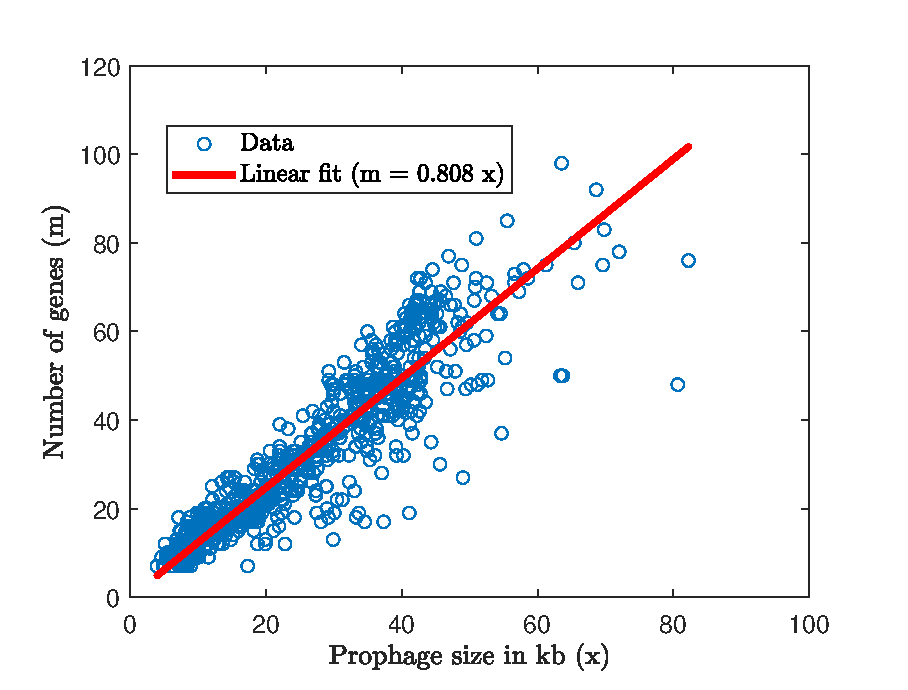
\includegraphics[scale=0.65]{genes}
\caption[Data showing the strong correlation between length of prophage and the number of genes on that prophage.]{Data from ACLAME database (\href{http://aclame.ulb.ac.be}{http://aclame.ulb.ac.be}), showing the strong correlation between length of prophage and the number of genes on that prophage.  All prophages in the database of length up to 85 kb were considered.}
\label{fig:genes}
\end{figure}

\subsection{Lysogeny}
The function $f(x)$ in Equation \ref{pde} represents the length distribution of prophages which enter bacterial genomes through lysogeny.  In other words, in the event that a phage genome will be integrated into a bacterial genome through lysogeny, $f(x)$ gives the probability density for the length of the phage genome to be integrated.  Thus, $f(x)$ captures not only the distribution of autonomous temperate phage genome lengths, but also any potential differences in lysogeny probabilities among these phages (see Appendix C for further details).

Most temperate phages are double-stranded (ds) DNA viruses \citep{szekely_single-stranded_2016}, although several single-stranded (ss) DNA phages have also been identified  as temperate \citep{krupovic_single-stranded_2015}.  We therefore expect that $f(x)$ might resemble the distribution of dsDNA phage lengths in nature.  Consistent with results reported for dsDNA phage (see Figure 1 in \cite{bobay_pervasive_2014}), we assume that the length distribution of these active phages may be multimodal, and that the minimum length for an autonomous phage is longer than the minimum length for a (possibly degraded and cryptic) prophage.  For convenience, we describe the multimodal distribution of active phages as the sum of $g =1$ to $3$ Gaussian probability density functions (i.e.\ a mixed distribution with up to three components):
\begin{eqnarray}\label{gs}
f(x) = \begin{cases} 
\sum_{i=1}^g {p_{i}e^{-\frac{(x-(\theta+\mu_{i}))^{2}}{\sigma_{i}^{2}}}} & x \geq \theta \\
0,  & x < \theta.
\end{cases}
\end{eqnarray}
where $p_{i} >0, \, \, \, \mu_{i} >0, \,\,\, \sigma_{i}>0$ for $i= 1$ to $g$ represent relative weights (in the convex combination), means and standard deviations of the component distributions, respectively. Note that $\theta$ in this expression gives the length of the smallest autonomous temperate phage. 
Temperate dsDNA phages have diverse genomes, with the smallest reported size of about $15$ kb (\textit{Bacillus phage Bam35c}) \citep{ravantti_comparative_2003, gaidelyte_linear_2005}; \cite{bobay_pervasive_2014} report that the smallest autonomous dsDNA phage that can infect enterobacteria is $30$ kb.  Here we assume that the smallest autonomous dsDNA phage that may successfully lysogenize a host has a genome size of $\theta = 20$ kb, however our results were not sensitive to this choice of threshold parameter (see Appendix B).

\subsection{Horizontal gene transfer (HGT)} 
HGT describes several processes by which genetic material is transferred from a donor bacterium to a recipient bacterium. The transfer of genetic material can be accomplished through \textit{conjugation}, \textit{transformation} and \textit{transduction}.  Although it has been inferred that transduction is 1000 times less likely than conjugation to transfer antibiotic resistance genes \citep{volkova_modeling_2014}, we note that transduction might be especially relevant to the HGT of chromosomal prophages.  In specialized transduction, a prophage erroneously excises from the bacterial genome, taking a neighboring piece of the host chromosome and possibly integrating an incomplete prophage sequence into the new bacterial host; in generalized transduction, DNA from elsewhere in the host chromosome (not necessarily adjacent to the prophage) is packaged into the viral capsid and transmitted to a new host \citep{touchon_embracing_2017}.  Since, for example, prophages can encode packaging-recognition sites (\textit{pac} signals) \citep{casjens_bacteriophages_2009}, transduction could play a significant role in the prophage size distribution. 

The function $g(x)$ in equation \ref{pde} represents the transfer of prophage sequences, or partial prophage sequences, into host genomes by any of these processes of HGT.  We reasoned that shorter DNA sequences should be transferred with higher probability than larger ones, therefore, we assume that $g(x)$ must be a non-negative decreasing function, i.e, $g(x) \geq 0$ and $g^{'}(x) \leq 0$ for all $x \in [0,x_M]$ (recalling that $x_M$ is the size of the largest prophage in the dataset).  The simplest function which satisfies these properties is a decreasing linear function, 
$g(x) = -x + x_M$.  The slope of this line is scaled by the free parameter $\beta$ representing the maximum rate of prophage integration via HGT.  We also investigated more complex functions describing HGT (data not shown) but these were not justified in data fitting. 

\subsection{Degradation} Mutational processes in bacterial genomes exhibit a strong bias toward deletion \citep{kuo_deletional_2009}, and mutational degradation may render intact prophages cryptic, i.e.\, incapable of induction or unable to form plaques.  Under the assumption that the probability of deletion is constant along the genome, we recover a linear relation between prophage sequence length and the rate of loss, $D(x) = r_{D}\,x,$ where again $x$ is the length of the prophage sequence in kb, and $r_{D}$ is the rate of degradation (kb of prophage sequence lost, per bacterial generation, per kb of prophage sequence).  Degradation from larger to smaller prophages depends on the gradient of the prophage length distribution, thus this process introduces an advective term.

\subsection{Selective advantage} \label{sel}
Integrated prophage often confer fitness benefits to their bacterial hosts \citep{bondy-denomy_when_2014}. Longer prophage sequences may encode a greater number of beneficial genes, conferring greater advantage to host cells and increasing the prophage population in turn. Let $n_b$ be the total number of potentially beneficial genes carried by phage. If $L$ is the number of genes in a prophage as it attaches to the bacterial genome, suppose after degradation $m$ intact genes remain. Then the probability, $\mathcal{P}(i),$ where $0< i \leq m,$ that the prophage of length $m$ carries  $i$ beneficial genes is 
\begin{eqnarray}
\mathcal{P}(i)= \frac{\binom{n_b}{i}\,\binom{L-n_b}{m-i}}{\binom{L}{m}}\nonumber,
\end{eqnarray}
which is a Hypergeometric distribution, with expected value $\sum_{i = 1}^{m}  i \,\mathcal{P}(i) = \frac{ n_b\,m}{L}$.  Converting this expectation to units of sequence length, a prophage degraded to length $x = m/\kappa$ from initial length $x_L = L/\kappa$ is expected to carry fraction $x/x_L$ of all possible beneficial genes (a result we will use in Equation \ref{sel1}). 


The probability that a prophage of length $x$ is a degraded version of an active phage of length $x_L$ is given by the proportion of active phages that have length $x_L$, as a fraction of all the active phages that might have given rise to this prophage:
\begin{eqnarray}\label{s1}
\mathcal{A}(x, x_L) = \begin{cases} 
0, & x > x_{L} \\
\dfrac{f(x_{L})}{\sum\limits_{y = \,x}^{x_{M}}f(y)},  & x \leq x_{L}.
\end{cases}
\end{eqnarray}
We assume that an active prophage confers an overall selective advantage $r_S$ per bacterial generation.  For mathematical tractability, we assume that the magnitude of this maximum selective effect does not vary with the initial length of the active phage sequence; this is a simplification that should be relaxed in future work.
We can then deduce $S(x)$, the expected fraction of $r_S$ that will be conferred by a prophage of length $x$, by conditioning and summing over all possible active phages that may have produced this prophage:
\begin{eqnarray}
\label{sel1}
S(x) = \sum\limits_{x_{L}=\,x}^{x_{M}} \mathcal{A}(x, x_{L})\frac{x}{x_{L}}.
\end{eqnarray}
Thus, the term $r_S S(x)$ gives the change in the intrinsic growth rate conferred on average by a prophage of length $x$.

Finally, we note that along with potential fitness benefits, prophage genes may also impose fitness costs on their hosts \citep{koonin_evolution_2009}.  The parameter $r_S$, which could be positive or negative, reflects the sum total of these costs and benefits.  Thus for example if the best-fit value of $r_S$ were negative, the model would predict that independent of induction, the carriage of prophage genes comes at a net cost to the host cell.

\subsection{Induction} \label{indu}
 Prophage may re-instigate the lytic life cycle, either spontaneously or in response to some stress, resulting in the death of the host cell and release of progeny phages.   As before, we let $L$ denote the number of genes in an active phage, while $m$ is the number of genes retained on a (possibly degraded) prophage.  Assume $n_l$ is the number of phage genes required for the loss of prophage from the bacterial genome through induction.  (Since the model tracks only the frequency of bacterial hosts carrying prophages of a given length, this loss could reflect either the excision of prophage from the bacterial genome, or the death of the bacterial host through lysis.)  The probability that a prophage carries the genes required for induction, given that after degradation it carries $m$ out of $L$ genes is:
\begin{eqnarray}
 \begin{cases} 
0, & m < n_l \\
\dfrac{\binom{L-n_l}{m-n_l}}{\binom{L}{m}},  & n_l \leq m \leq L.
\end{cases}\nonumber
\end{eqnarray}
We again use the parameter  $\kappa$ to convert between gene number and sequence length, and make use of  Stirling's approximation to simplify factorial terms.  We thus approximate the probability that a prophage, initially of length  $x_{L}$ but degraded to length $x$, contains the genes required for induction as:
\begin{eqnarray}
\mathcal{R}(x,x_L)\approx
 \begin{cases} 
0, & x < x_n \\
\dfrac{x^{\kappa \, x}\, (x_{L}-x_{n})^{\kappa (x_{L}-x_{n})}}{ x_{L}^{\kappa\, x_{L}}{(x- x_{n})}^{\kappa (x- x_{n})}},  &x_{n} < x \leq x_{L},
\end{cases}
\end{eqnarray}
where $x_n = n_l/\kappa$ is the length of the genes required.
The probability that a prophage of length $x$ is a degraded version of prophage of length $x_{L}$ is given by (\ref{s1}).
Thus, the overall probability that the prophage contains the genes required for induction (excision from the host genome), after conditioning and summing over all possible active phages that may have produced this prophage is given as:  
\begin{eqnarray}\label{ind}
I(x) \approx \sum \limits_{x_{L}=\,x}^{x_{M}}\mathcal{A}(x, x_{L})\,\mathcal{R}(x, x_{L}).
\end{eqnarray}
The parameter $r_I$ gives the induction rate, that is, the rate per prophage per bacterial generation at which prophages are lost from bacterial genomes due to induction.  Finally, we note that because prophages lost to induction may or may not contain the genes required for re-infection, we do not expect that the product $I(x) P(x)$ will directly yield the distribution of lysogenizing phages, $f(x)$ (but see Appendix C). 

Typical geometries of these five functions -- lysogeny, HGT, degradation, selection and induction -- are illustrated in Figure ~\ref{fig:func}.

\begin{figure}[htb!]
\captionsetup[subfigure]{labelformat=empty}
\begin{subfigure}[t]{0.5\textwidth}
\centering
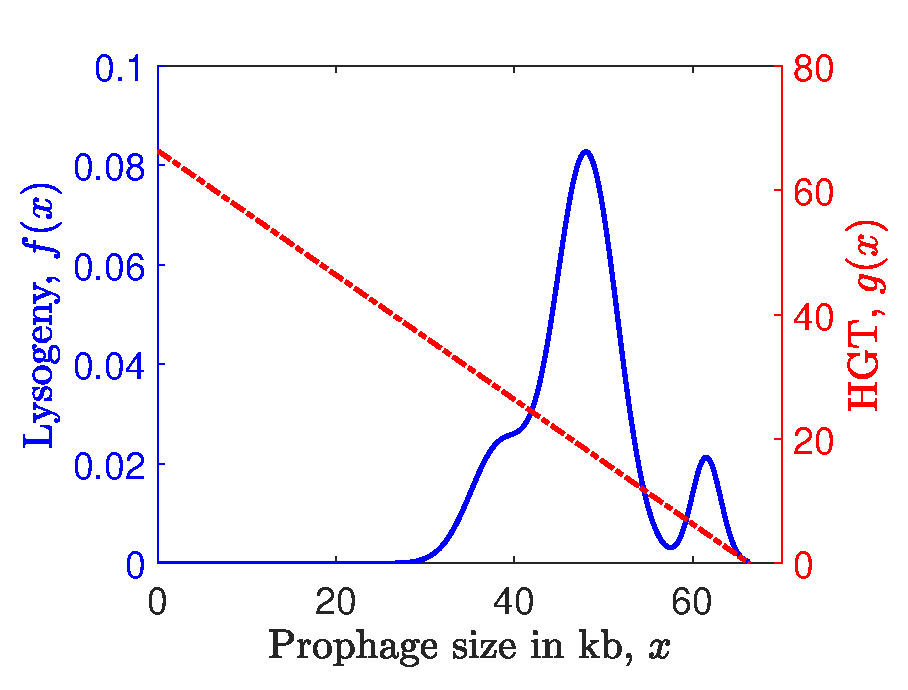
\includegraphics[scale=0.5]{phage1.eps}
\subcaption[subfigcapskip = 50pt]{}

\end{subfigure}\hfill
\begin{subfigure}[t]{0.5\textwidth}
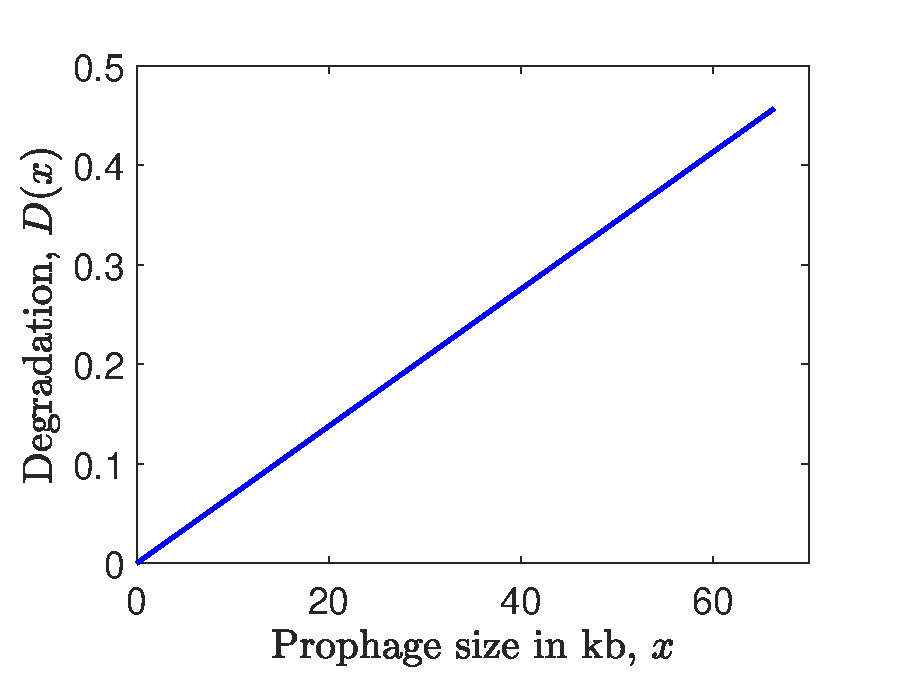
\includegraphics[scale=0.5]{deg2.eps}
            \subcaption[subfigcapskip = 50pt]{}
            
\end{subfigure} 
\begin{subfigure}[t]{0.5\textwidth}
\centering
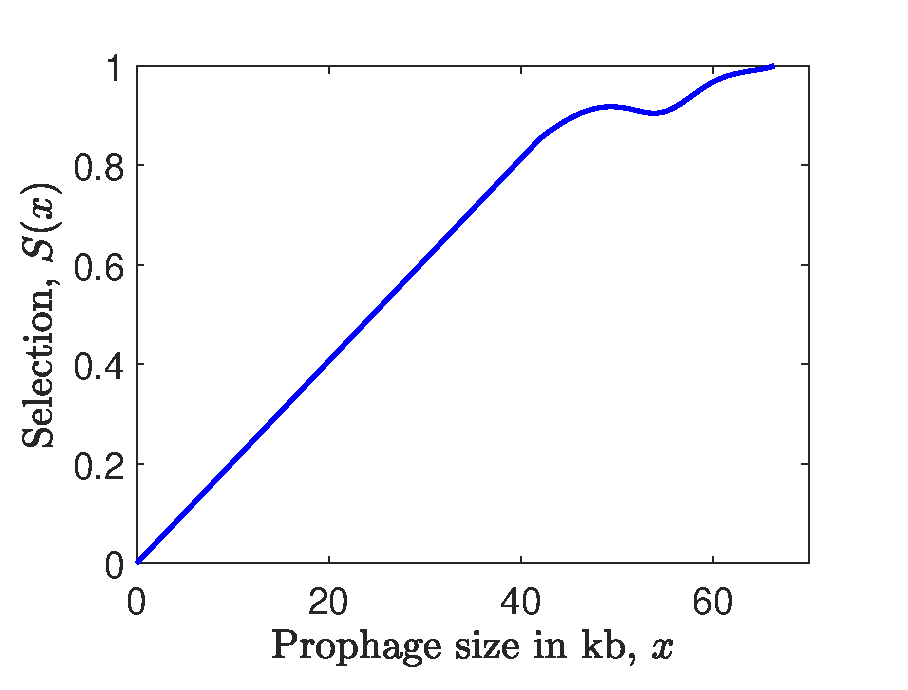
\includegraphics[scale=0.5]{sel3.eps}
\subcaption[subfigcapskip = 50pt]{}

\end{subfigure}
\begin{subfigure}[t]{0.5\textwidth}
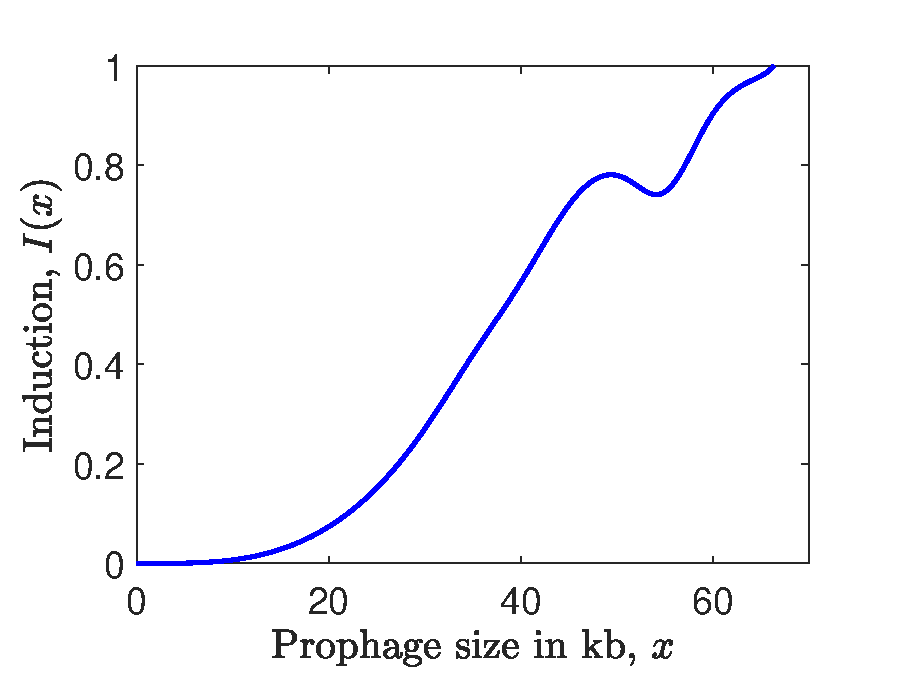
\includegraphics[scale=0.5]{ind4.eps}
\subcaption[subfigcapskip = 50pt]{}
\end{subfigure}
\caption[Example geometries of the influx distributions via lysogeny and HGT, as well as the degradation, selection and induction functions.]{Example geometries of the influx distributions via lysogeny and HGT (top panel, left and right axes respectively), as well as the degradation, selection and induction functions, plotted against prophage size. To illustrate the shapes of these functions, we have used parameters corresponding to the best fit to Data Set 1 (see Results to follow). Parameter values are $p_{1} = 17.95, \, \mu_{1} = 18.37, \, \sigma_{1} = 4.73,$ $p_{2} = 64.19, \, \mu_{2} = 28.06, \, \sigma_{2} = 4.93$, $p_{3} = 16.57, \, \mu_{3} = 41.54, \, \sigma_{3} = 2.32,$ $r_{D} = 0.0069$. }\label{fig:func}
\end{figure}
%%%%%%%%%%%%%%%%%%%%%%%%%%%%%%%%%%%%%%%%%%%%%%%%%%%%%%%%%%%%%%%%%%%%%%%%%%%%%%%%%%%%%%%%%%%
\subsection{Closed-form solution}

If we consider $\lim_{t \to \infty}\,Q(x, t)=P(x)$ and  $D(x) = r_{D}\,x$
then the differential equation generating the steady state solution of equation \ref{pde} is given by \begin{eqnarray}\label{appsol}
 \frac{d P(x) }{d x}+ \left(\frac{1}{x}+\mathcal{F}(x)\right)\,P(x)+\frac{\alpha}{r_{D}\, x} \, f(x)  + \frac{\beta}{r_{D}\,x} \, g(x) =0
\end{eqnarray}
where $\mathcal{F}(x) = (r_S\, S(x) - r_I\, I(x))/(r_D\,x)$.
Equation (\ref{appsol}) is first order linear ordinary differential equation and its solution is given by 
\begin{eqnarray}\label{ssol}
 P(x) &=&\frac{-\,e^{-\int{\mathcal{F}}(x)dx} }{r_D\, x}\,\int{(\alpha \,f(x)\, + \, \beta\, g(x))\,e^{\int{\mathcal{F}}(x)dx}dx}+\frac{C}{x}\, e^{-\int{\mathcal{F}}(x)dx},
\end{eqnarray}
where $C$ is a constant of integration.  Although in general a numerical approach is required to evaluate $P(x)$ due to the complexity of the functions $S(x)$, $I(x)$ and $f(x)$, the form of this solution will prove valuable in eliminating some solutions during model selection (see Table \ref{table:30} below).


\section{Model selection and data fitting}\label{ns}
Although lysogeny, HGT, degradation, selection and induction may all contribute to the maintenance of the prophage population in nature, we performed rigorous model selection to determine which of these processes are statistically justified in modeling the data.  This approach allows us to identify the key evolutionary processes underlying the prophage distribution, and to estimate the relative magnitude of their effects.

Since lysogeny is a necessary prerequisite for the prophage distribution, we considered  models that included incoming prophage ($f(x)$) but included or excluded HGT, degradation, induction and selection in all possible combinations.  Thus in total, we tested all $2^4 = 16$ possible models.  For brevity, Table \ref{table:30} lists the full model, as well as all possible models that exclude HGT; analogous models including HGT were also tested.  
\renewcommand{\baselinestretch}{1}

\begin{table}[htbp]
\centering
\begin{tabular}{ p{1cm}p{2cm}p{10.2cm}}
\hline
Model & Processes & Steady-state solution, $P(x)$\\
 & $f\,D\,I\,S \, g$  & \\
\hline
\\
1 & \checkmark \checkmark \checkmark \checkmark \checkmark& $\frac{-\,e^{-\int{\mathcal{F}}(x)dx} }{r_D\, x}\,\int{(\alpha \,f(x)\, + \, \beta\, g(x))\,e^{\int{\mathcal{F}}(x)dx}dx}+\frac{C}{x}\, e^{-\int{\mathcal{F}}(x)dx}$\\
\\
\hline
\\
2 & \checkmark \checkmark \checkmark \checkmark \ding{55}& $\frac{-\alpha \,\,e^{-\int{\mathcal{F}}(x)dx} }{r_D\, x}\,\int{f(x)\,e^{\int{\mathcal{F}}(x)dx}dx}+\frac{C}{x}\, e^{-\int{\mathcal{F}}(x)dx}$\\
\\
\hline
\\
3& \checkmark \ding{55} \checkmark \checkmark \ding{55}& $\frac{-\alpha f(x)}{S(x)-I(x)}$ where $S(x)\neq I(x)$\\
\\
\hline
\\
4& \checkmark  \checkmark \ding{55} \checkmark \ding{55}& \small{$-\frac{\alpha}{r_{D}}\frac{1}{x}e^{-\int \left(\frac{r_{S}}{r_{D}}\frac{S(x)}{x}\right)dx}\int f(x)e^{\int \left(\frac{r_{S}}{r_{D}}\frac{S(x)}{x}\right)dx}dx+\frac{C}{x}e^{-\int \left(\frac{r_{S}}{r_{D}}\frac{S(x)}{x}\right)dx}$}\\
\\
\hline
\\
5 & \checkmark  \checkmark \checkmark \ding{55} \ding{55} & $ -\frac{\alpha}{r_{D}}\frac{1}{x}e^{\int \left(\frac{r_{I}}{r_{D}}\frac{I(x)}{x}\right)dx}\int f(x)e^{-\int \left(\frac{r_{I}}{r_{D}}\frac{I(x)}{x}\right)dx}dx+\frac{C}{x}e^{\int \left(\frac{r_{I}}{r_{D}}\frac{I(x)}{x}\right)dx}$\\
\\
\hline
\\
6& \checkmark  \checkmark \ding{55} \ding{55} \ding{55}& $-\frac{\alpha}{r_{D}\,x}\int  f(x)dx+\frac{C}{x}.$\\
\\
\hline
\\
7& \checkmark  \ding{55} \checkmark \ding{55} \ding{55}& $\frac{\alpha f(x)}{I(x)},$ where $I(x)\neq 0.$\\
\\
\hline
\\
8 & \checkmark  \ding{55} \ding{55} \checkmark \ding{55}& $\frac{-\alpha f(x)}{S(x)},$ where $S(x) \neq 0.$\\
\\
\hline
\\
9 & \checkmark \ding{55} \ding{55} \ding{55} \ding{55}&
no steady-state solution\\
\\
\hline
\end{tabular}
\caption[A detailed description of the models considered.]{A detailed description of the models considered. Each model includes or excludes terms on the right-hand side of Equation \ref{pde} as indicated.  The analytical forms for the steady-state solutions, as shown in the right-most column, allow us to eliminate several models from further analysis (see text for details).
Here $\mathcal{F}(x) = \frac{r_S\, S(x)}{r_D\,x }- \frac{r_{I}\, I(x)}{r_D\, x}$ and $C$ is an arbitrary constant.}
\label{table:30}
\end{table}
%\end{landscape}

%\renewcommand{\baselinestretch}{2}

The first step in analyzing these models was to exclude models that are qualitatively unable to capture the prophage size distribution data. 
From the analytical solutions of models 3 (with both induction and selection present), 7 (with only induction present), and 8 (with only selection present), we see that in these cases, the steady-state solution $P(x)=0$ wherever the 
incoming phage distribution $f(x)=0$.  Thus these models predict the absence of prophage with lengths smaller than $\theta = 20$ kb.  These models are clearly unable to capture the distributions illustrated in Figure \ref{fig:data} and were excluded from further analysis.  This result makes intuitive sense: the three excluded models do not include degradation, and therefore cannot explain prophage with lengths shorter than the lengths of autonomous temperate phage.

We proceeded with model selection using the remaining five models (models 1, 2, 4, 5 and 6), fitted to each data set. For each model, we also allowed the function $f(x)$ (the incoming phage distribution) to be described by a mixed distribution incorporating one to three Gaussian distributions.  While the data sets included between $n$ = 128 and $n$ = 737 data points, the tested models included between $k$ = 4 and $k$ = 15 free parameters.  We used a finite difference scheme to obtain, numerically, the steady-state solution to the model, and compared this steady-state solution to the data, optimizing the log-likelihood to identify the best fit parameter values. The log-likelihood is defined as $\log(L) = \sum \log P(x_{i})$, 
where $x_{i}$ are the $n$ observed lengths of prophage sequences in the data set, $P(x)$ is the numerically obtained steady-state solution, and the sum is taken for $i = 1 \, \text{to} \, n$.
 To select the best model among the candidate models, we used the  Akaike Information Criterion (AIC) \citep{akaike_likelihood_1981}, defined as:
\begin{eqnarray}\label{aic}
\mbox{AIC} =2k -2\,\log\left(\hat{L}\right)
\end{eqnarray}
where $k$ is the number of free parameters, and $\log\left(\hat{L}\right)$ is the maximum log-likelihood. 

While the lowest AIC value corresponds to the best fit, it is possible that several candidate models may offer equivalently good fits; these correspond to models that cannot be rejected, statistically.  To address this issue, we compute the relative probability. If $AIC_{min}$ is the lowest $AIC$ value obtained for one of the candidate models, the relative probability \citep{burnham_model_2003} is defined for each candidate model as $R = \exp\left(\, ({AIC_{min}-AIC})/2\,\right)$.
The best fit model will thus have relative probability 1. If we imagine adding a single ``dummy" variable to the best fit model, that is, we add an additional parameter that has no effect on the fit, the AIC will increase by 2 and the log-likelihood will not change.  Thus the relative probability of the best fit model including an extra dummy parameter will be $\exp(-1) = 0.368$. We therefore reject candidate models with $R \leq \exp(-1)$.  If candidate models have relative probability values that exceed $\exp(-1)$, we are unable to reject them and consider them as possible ``best fits” to the data. 
%%%%%%%%%%%%%%%%%%%%%%%%%%%%%%%%%%%%%%%%%%%%%%%%%%%%%%%%%%%%%%%%%%%%%%%%%%%%

\section{Results}
\label{results}
We fit models 4, 5 and 6 to each of the three data sets, including in each model the possibility of up to three components in the incoming phage distribution, $f(x)$, and including or excluding HGT, $g(x)$.  
A full summary of the model-fitting results is provided in Appendix \ref{a2} (Table \ref{table:bob}, Table \ref{table:desu}, Table \ref{table:aclame} for Data Sets 1, 2 and 3, respectively).

Despite the reduced number of free parameters in the simpler models (an attribute rewarded by the AIC criterion), in no case did models 4 (degradation and selection), 5 (degradation and induction) or 6 (degradation) achieve the best fit to any of the data sets.  To illustrate, we have reproduced the fits obtained to Data Set 1 with these three models in Figure \ref{fig:noBi}.
\begin{figure}[H]
\centering
  \begin{subfigure}[t]{0.3\textwidth}
  \centering
 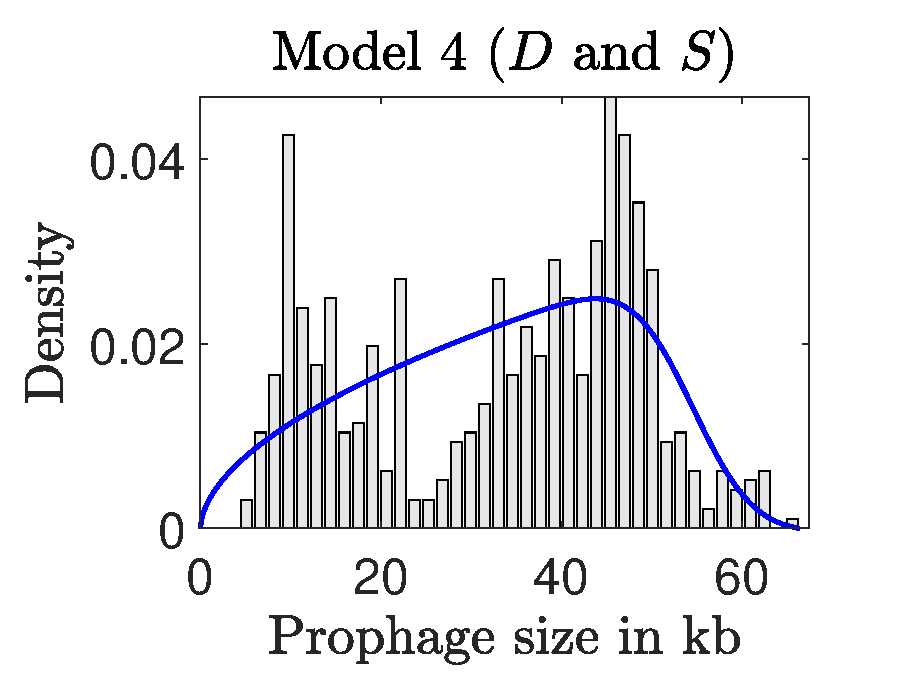
\includegraphics[scale=0.40]{DegSel.eps}
 %\subcaption[subfigcapskip = 50pt]{Model 4 ($D$ and $S$).}
% \label{fig:DegSel}
 \end{subfigure}\hfill
 \quad
 \begin{subfigure}[t]{0.3\textwidth}
 \centering
 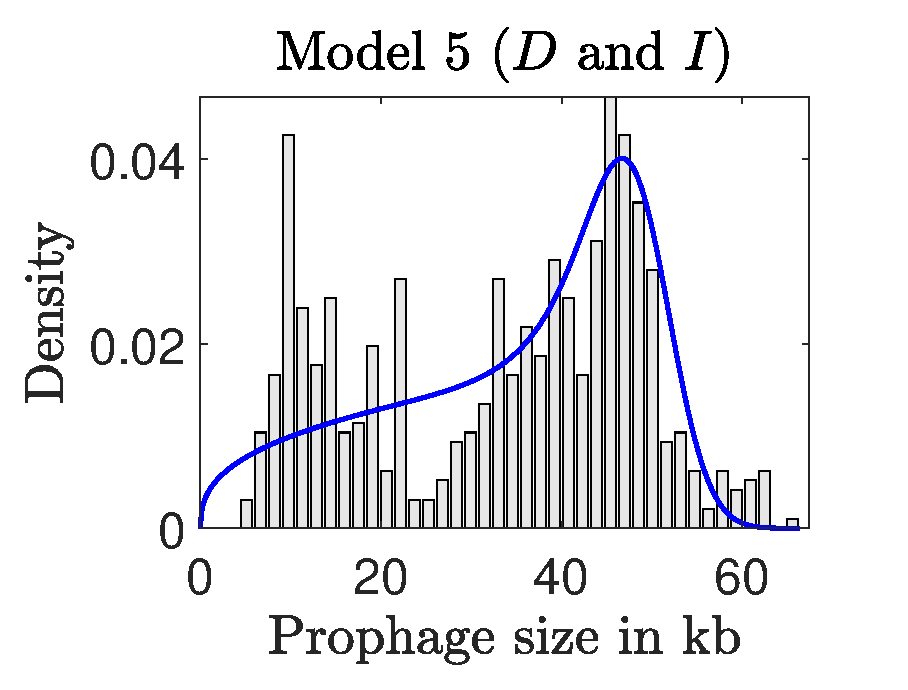
\includegraphics[scale=0.40]{DegInd.eps}
 %\subcaption[subfigcapskip = 50pt]{Model 5 ($D$ and $I$).}
 \label{fig:DegInd}
 \end{subfigure}\hfill
 \quad
 \begin{subfigure}[t]{0.3\textwidth}
  \centering
 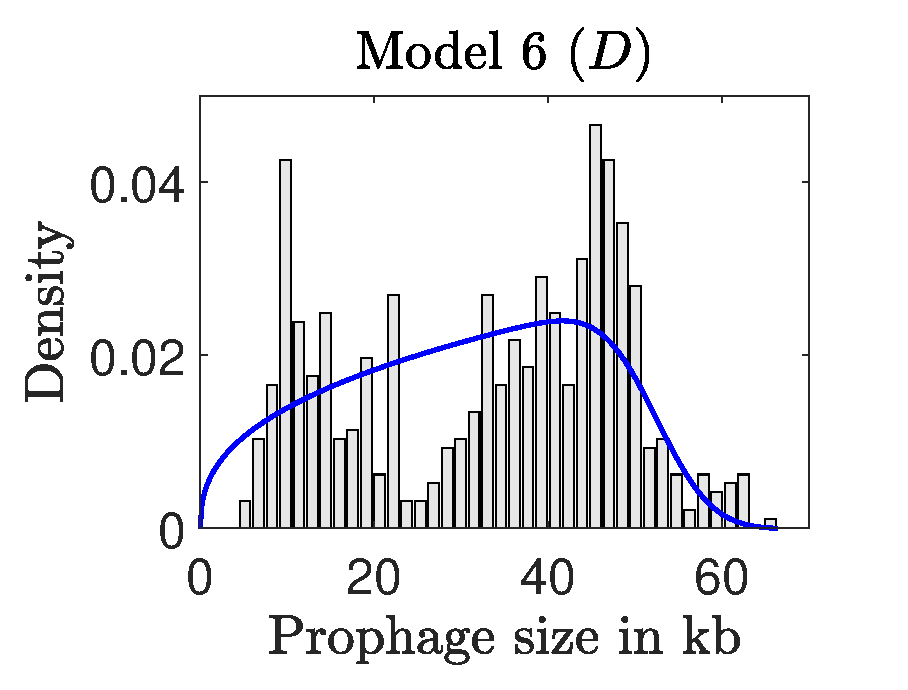
\includegraphics[scale=0.40]{onlyDeg.eps}
 %\subcaption[subfigcapskip = 50pt]{Model 6 ($D$).}
 \label{fig:Deg}
 \end{subfigure}
  \caption[Lines of best fit obtained to Data Set 1 by models 4, 5 and 6.]{ Lines of best fit ($P(x)$, shown in blue) obtained to Data Set 1 (histograms) by models 4, 5 and 6 (see Table \ref{table:30}); these models did not provide adequate fits to the data.}
\label{fig:noBi}
\end{figure}

 For all three data sets, then, model 2, as described by Equation \ref{pde} with $\beta =0$, provided the best fit, with varying degrees of complexity in the function describing the incoming phage distribution ($f(x)$).  We describe and illustrate these results below.

\subsection{Data Set 1}
 The best fit to these data from {\it E.~coli} and {\it S.~enterica} was obtained using the full model without HGT (model 2), with the distribution of incoming phages described by a mixture of three underlying Gaussian distributions ($g=3$).  This model has 14 free parameters (see Figure~5A). The second-best fit is the same model with HGT; this fit has relative probability 0.372 and thus cannot be rejected.  We note however that the contribution of HGT in this second-best fit is very small (see Table \ref{table:res}).  The best fits are illustrated in Figure~5B and 5C. Detailed results of data fitting are provided in
Table \ref{table:bob}, Appendix \ref{a2}.
%%%%%%%%%%%%%%%%%%%%%%%%%%%%%%%%%%%%%%%%%%%%%%%%%
\begin{figure}[H]
\begin{subfigure}[t]{0.3\textwidth}
\centering
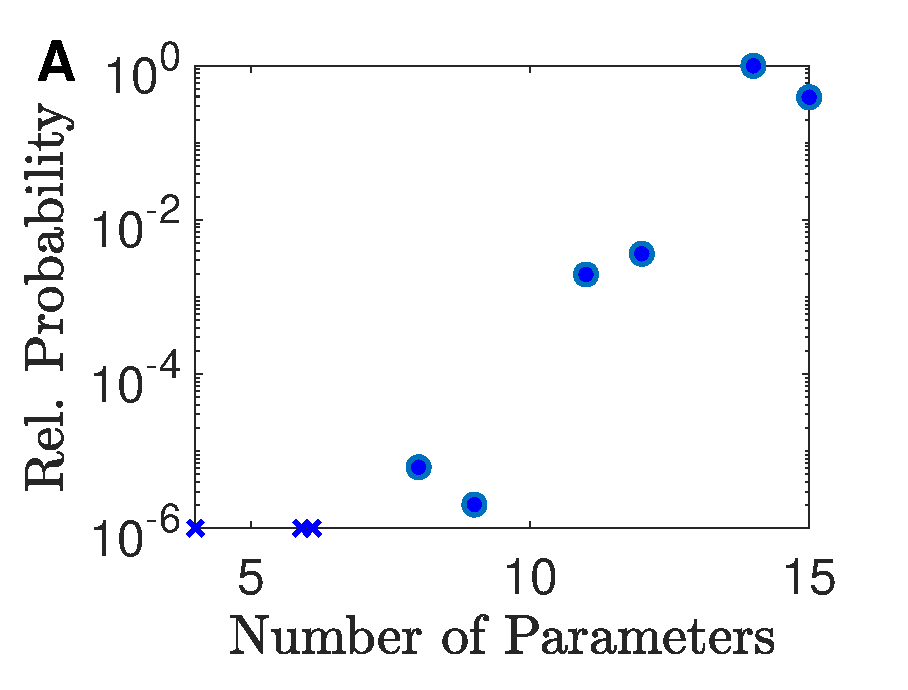
\includegraphics[scale=0.4]{bob_rel.eps}
%\subcaption[subfigcapskip = 50pt]
%\label{fig:bob_rel}
\end{subfigure}\hfill
\begin{subfigure}[t]{0.3\textwidth}
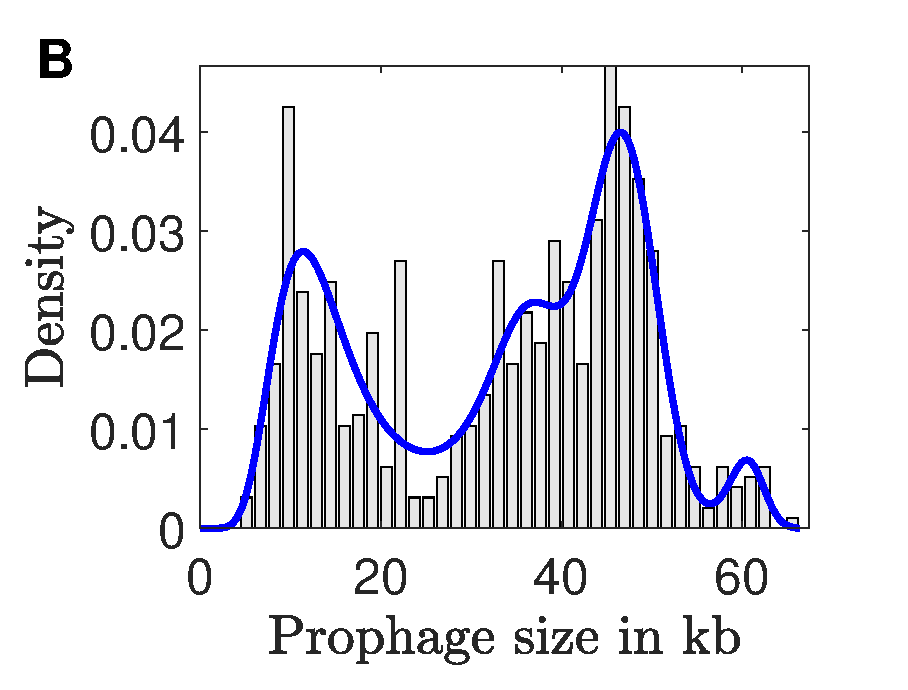
\includegraphics[scale=0.4]{bob_best_pdf.eps}
            %\subcaption[subfigcapskip = 50pt]{%Best fit.
%            }
            %\label{fig:bob_bestpdf}
\end{subfigure}\hfill
\begin{subfigure}[t]{0.3\textwidth}
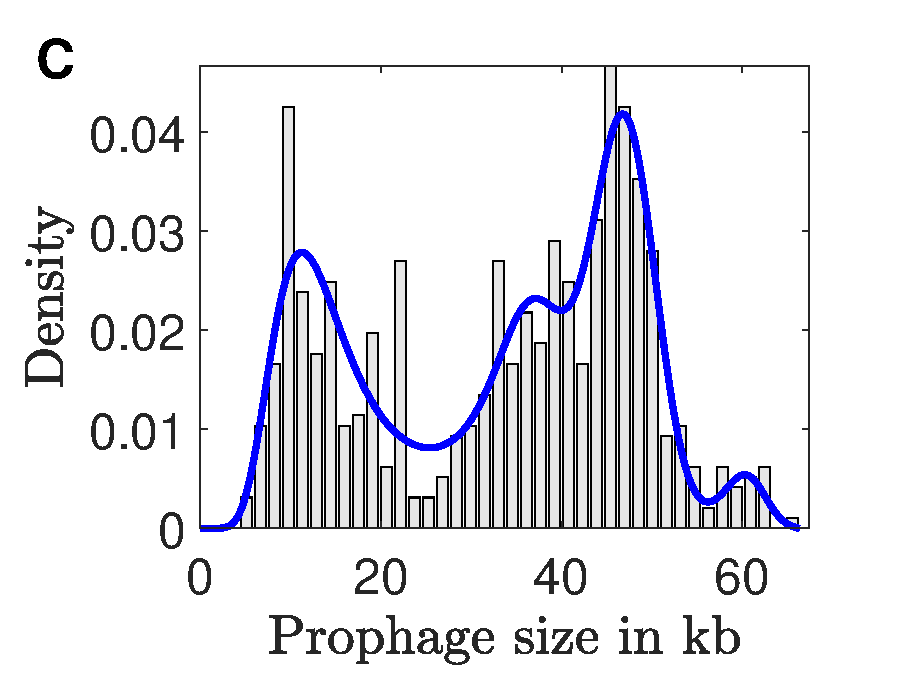
\includegraphics[scale=0.4]{bob_best2_pdf.eps}
%\subcaption[subfigcapskip = 50pt]
 %\label{fig:bob_best2_pdf}
 \end{subfigure}\hfill
\caption[Model fitting results for Data Set 1.]{ Model fitting results for Data Set 1.  (A) The relative probability of candidate models for Data Set 1, plotted as a function of the number of parameters in that model; crosses indicate relative probabilities $\leq 10^{-6}$. (B) The best fit predicted by the model ($P(x)$, blue curve) to Data Set 1 (histogram). The best fit included 14 free parameters. (C) The second-best fit  model (blue curve) to Data Set 1 (histogram). The second-best fit included 15 free parameters.}
\end{figure}
%%%%%%%%%%%%%%%%%%%%%%%%%%%%%%%%%%%%%%%%%%%%%%%%%%%%%%%%%%%%%%%%%%%%%%%%%%%%%%%%%%%%%%%%%%%%%%%%%%%%%%%%%%%%%%%%%%%%
\subsection{Data Set 2} 
The prophage length distribution from {\it Desulfovibrio} was best described by the full model without HGT, and a single Gaussian describing the incoming phage lengths ($g=1$, 8 parameter model), see Figure~6A.
This fit is illustrated in Figure~6B. Details are provided in Table \ref{table:desu} in Appendix \ref{a2}. 
%%%%%%%%%
\begin{figure}[H]
 \begin{subfigure}[t]{0.5\textwidth}
\centering
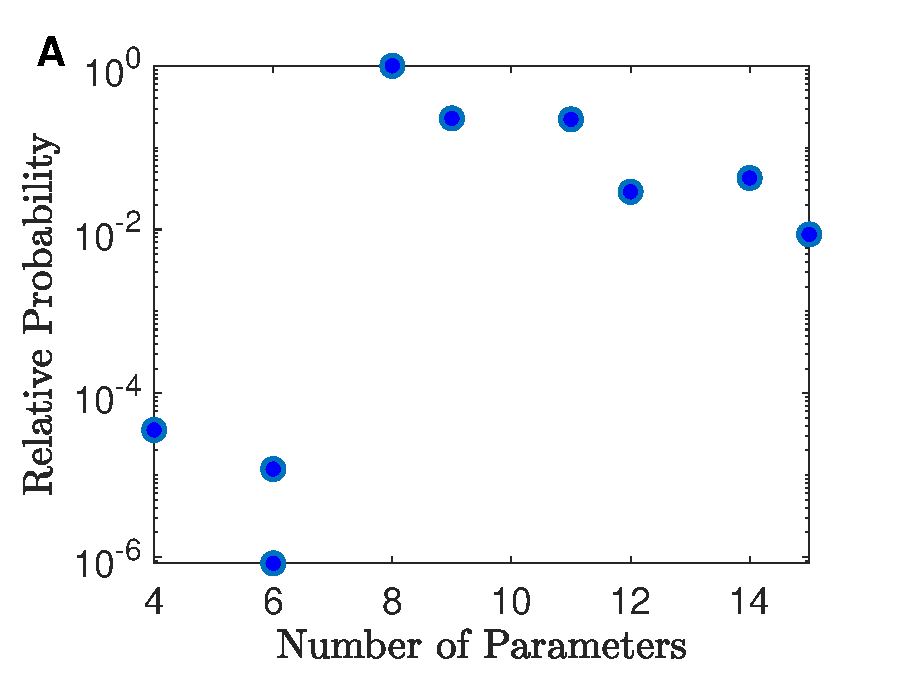
\includegraphics[scale=0.5]{desu_rel.eps}
%\subcaption[subfigcapskip = 50pt]{}
%\label{fig:desu_rel}
\end{subfigure}\hfill
\begin{subfigure}[t]{0.5\textwidth}
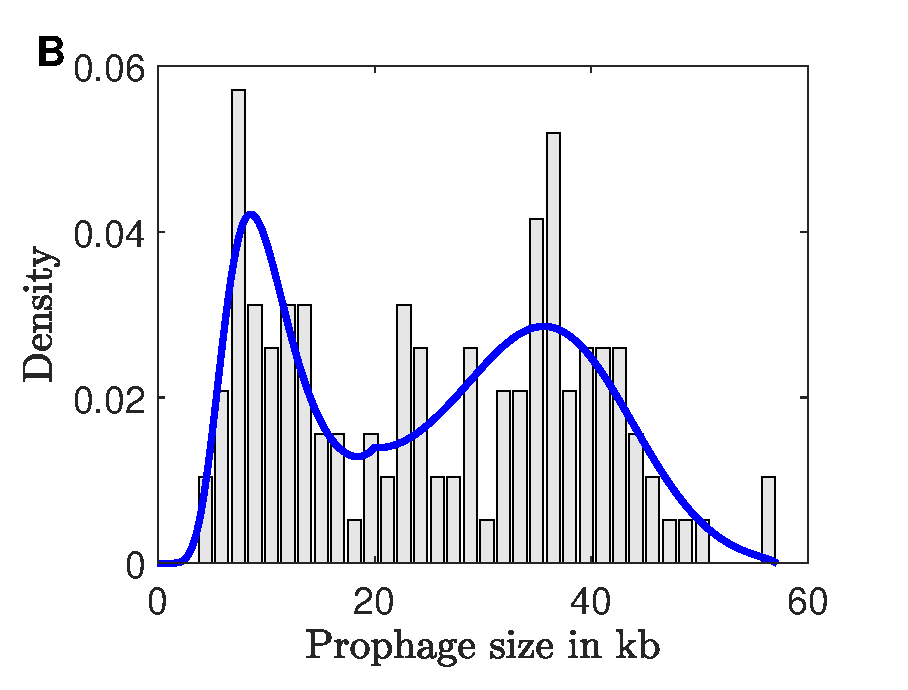
\includegraphics[scale=0.5]{desu_best_pdf.eps}
            %\subcaption[subfigcapskip = 50pt]{}
            %\label{fig:desu_bestpdf}
\end{subfigure}\hfill
\caption[Model fitting results for Data Set 2.]{ Model fitting results for Data Set 2. (A) The relative probability of candidate models for Data Set 2, plotted as a function of the number of parameters in that model.  (B) The best fit predicted by the model ($P(x)$, blue curve), to Data Set 2 (histogram). The best model includes 8 free parameters and has relative probability 1. 
}
\end{figure}
%%%%%%%%%%%%%%%%%%%%%%%%%%%%%%%%%%%%%%%%%%%%%%%%%%%%%%%%%%%%%%%%%%%%%%%%%%%%%%%%%%%%%%%%%%%%%%%%%%%%%%%%%%%%%%%%%%
\subsection{Data Set 3} 
The prophage length distribution from the ACLAME database was also best described by the full model with a single Gaussian describing incoming phage ($g=1$, 8 parameter model), see Figure~7A.
The best fit is illustrated in
Figure~7B.
Model fitting details are provided in Table \ref{table:aclame} in Appendix \ref{a2}. 
%%%%%%%%%%%%%%%
\begin{figure}[H]
 \begin{subfigure}[t]{0.5\textwidth}
\centering
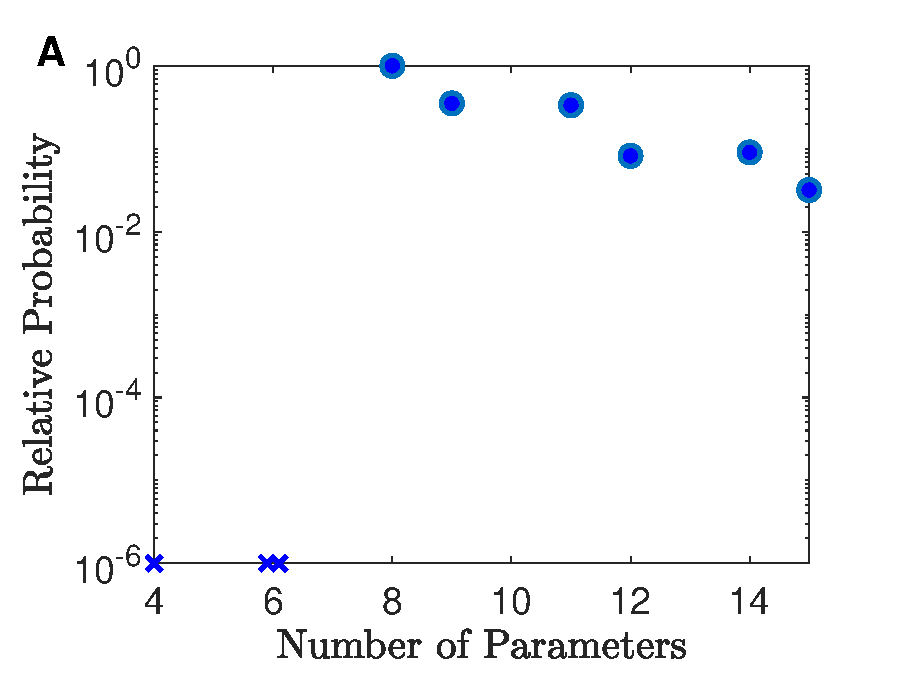
\includegraphics[scale=0.5]{aclame_rel.eps}
%\subcaption[subfigcapskip = 50pt]{}
%\label{fig:aclame_rel}
\end{subfigure}\hfill
\begin{subfigure}[t]{0.5\textwidth}
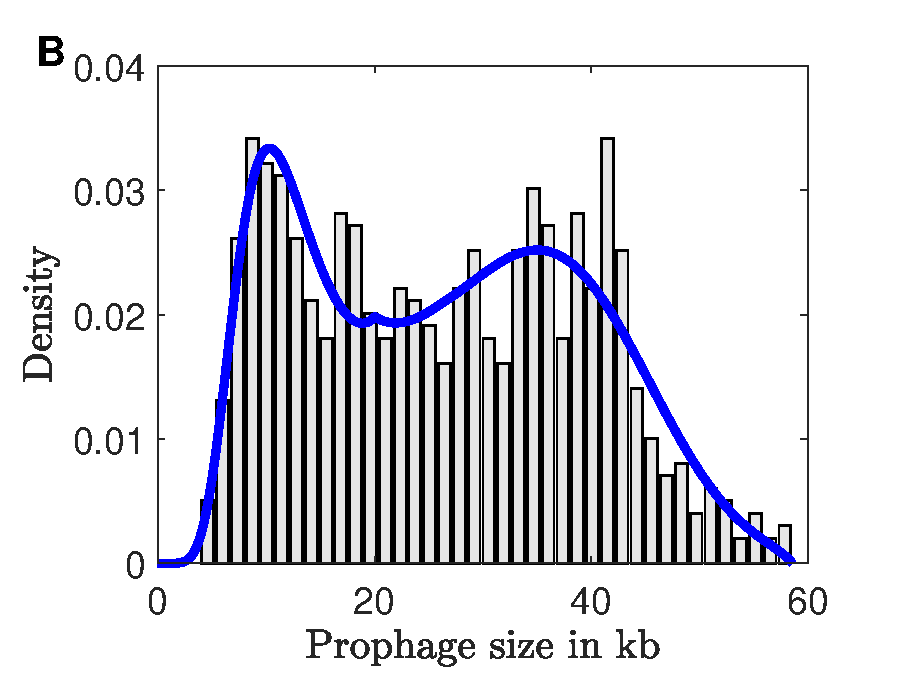
\includegraphics[scale=0.5]{aclame_best_pdf.eps}
            %\subcaption[subfigcapskip = 50pt]{}
            %\label{fig:aclame_bestpdf}
\end{subfigure}\hfill
\caption[Model fitting results for Data Set 3.]{ Model fitting results for Data Set 3. (A) The relative probability of candidate models for Data Set 3, plotted as a function of the number of parameters in that model; crosses indicate relative probabilities $\leq 10^{-6}$.
 (B) The best fit predicted by the model ($P(x)$, blue curve), to Data Set 3 (histogram). The best model includes 8 free parameters and has relative probability 1. 
}
\end{figure}

Table \ref{table:res} provides a summary of the best-fit parameter values obtained for the three data sets.  A sensitivity analysis, using Data Set 1, indicates a high degree of confidence in the parameter values, that is, all parameters are well-constrained by the data (see Appendix B).  However some care must be taken in interpreting these numerical values.  We present these rates in comparable units and address the implications of the quantitative results further in the Discussion.

%\renewcommand{\baselinestretch}{1}

% Table generated by Excel2LaTeX from sheet 'Sheet1'
%\begin{landscape}
\begin{table}[htbp]
%\renewcommand{\baselinestretch}{1}
  \centering
   \begin{tabular}{ p{0.5cm}>{\raggedright\arraybackslash}p{4.2cm}p{1.4cm}p{1.4cm}p{1.4cm}p{1.4cm}p{1.4cm}p{1.4cm}}
 \hline
 & & \multicolumn{2}{c}{Data Set 1}& \multicolumn{1}{c}{Data Set 2}& \multicolumn{1}{c}{Data Set 3} & \\
\multicolumn{2}{c}{\bf Parameter}  & best & 2\textsuperscript{nd} best &  &  & \multicolumn{1}{c}{\bf Mean$^\dag$}\\
 \hline
 $\alpha $   & Relative rate of lysogeny   & 0.1301  & 0.1982 & 0.1191 & 0.0734 & 0.1175\\
 \\
  $r_D$   & Relative rate of degradation   &0.0069  &0.01361& 0.0051 & 0.0052 & 0.0066\\
 \\
 $r_S$ &   Relative selection coeff. (intact prophage) &0.3137  & 0.7276 & 0.2397 & 0.2249 & 0.3110 \\
 \\
 $r_I$    & Relative rate of induction &0.6169 & 1.1139 & 0.5291 & 0.4713 & 0.6025\\
 \\
 $n_l$ &  Number of genes required for induction
 &2.440  &1.9512 & 2.440  & 2.5856  & 2.4198 \\
 \\
 $\beta$ & Relative rate of horizontal gene transfer & ----& $8.76 \times 10^{-13}$  & ---- & ---- & $8.76 \times 10^{-13}$\\ 
  \hline
\end{tabular}
    \caption[Parameter values for the best fits.]{Parameter values for the best fits. $^\dag$Mean across all data sets, weighted by relative probability for Data Set 1.}
    \label{table:res}%
\end{table}%
%\renewcommand{\baselinestretch}{2.0}

\section{Discussion}
\label{discussion}

Because we can only fit the steady-state solution of Equation \ref{pde} to the data, the resulting rates are only meaningful relative to other rates in the model.
Thus, although the time units of the best-fit rates are an arbitrary number of generations, we can express each of these rates relative to the induction rate.  This allows us to compare the evolutionary forces at play in terms of what we will call the ``expected prophage lifetime", that is, the average time between lysogeny and induction, for prophages that retain all the genes necessary for induction.  We find that the time between lysogeny events (new prophages entering the genome) is about 5 prophage lifetimes, while the selection coefficient, for an intact prophage, is approximately 0.5 per prophage lifetime.  If a prophage remains in the host genome for 100 bacterial generations before induction, for example, this selection coefficient would correspond to a selection coefficient $s=0.004$ per bacterial generation.  Finally, we predict that degradation of the prophage genome occurs at a rate of about 0.01 kb per kb in the prophage genome, per prophage lifetime.  Thus on average the model predicts that prophages have lost only 1\% of their genome to degradation at the time of induction.  These normalized rates are presented in summary in Table \ref{tab:rates}.

%\renewcommand{\baselinestretch}{1.0}

\begin{table}[H]
%\renewcommand{\baselinestretch}{1.0}
\centering
    \begin{tabular}{l r}
\hline
    \multicolumn{2}{c}{{ Rates expressed per expected prophage lifetime}}\\
    \hline
    {\bf Lysogeny} & 0.20\\
rate at which new prophage enters genome &  \\ 
{\bf Degradation}  & 0.01 \\
kb lost per kb of prophage genome &  \\
{\bf Selection} & 0.52 \\
overall selection coefficient per prophage lifetime & \\
{\bf Induction} & 1.00 \\
rate at which fully competent prophage induces & \\
\hline
    \end{tabular}
    \caption[Rates of the processes in the model, normalized by the induction rate. ]{Rates of the processes in the model, normalized by the induction rate.  Induction rate and selection coefficient are provided for fully intact (non-degraded) phage.  See text for details.}
    \label{tab:rates}
\end{table}

%\renewcommand{\baselinestretch}{2.0}


From these normalized rates, a picture emerges in which induction is the dominant fate for active prophages, occurring at a much higher rate than any other process.  New prophages enter the bacterial genome, on average, at a rate that is about one fifth of the induction rate.  These new sequences degrade very slowly relative to their induction rate, an observation that seems reasonable given that prophages would be unable to induce if degradation were rapid.   Despite the slow degradation rate, over evolutionary time smaller and smaller prophages accrue in host genomes.  These are maintained due to the balance between two effects: induction and selection.  In particular, short prophage sequences typically lack the genes required for excision or induction, but may still confer some benefit to their host.

Thus, our model predicts that the peak on the right of the prophage size distribution is due to the contribution of autonomous free phage, entering bacterial genomes via lysogeny, the term $\alpha f(x)$ in our model.  In contrast, the peak on the left is maintained in the region for which $r_s S(x) > r_I I(x)$, that is, where the benefits of selection outweigh the costs of induction, as illustrated in Figure ~\ref{fig:combine}.

\begin{figure}[H]
\centering
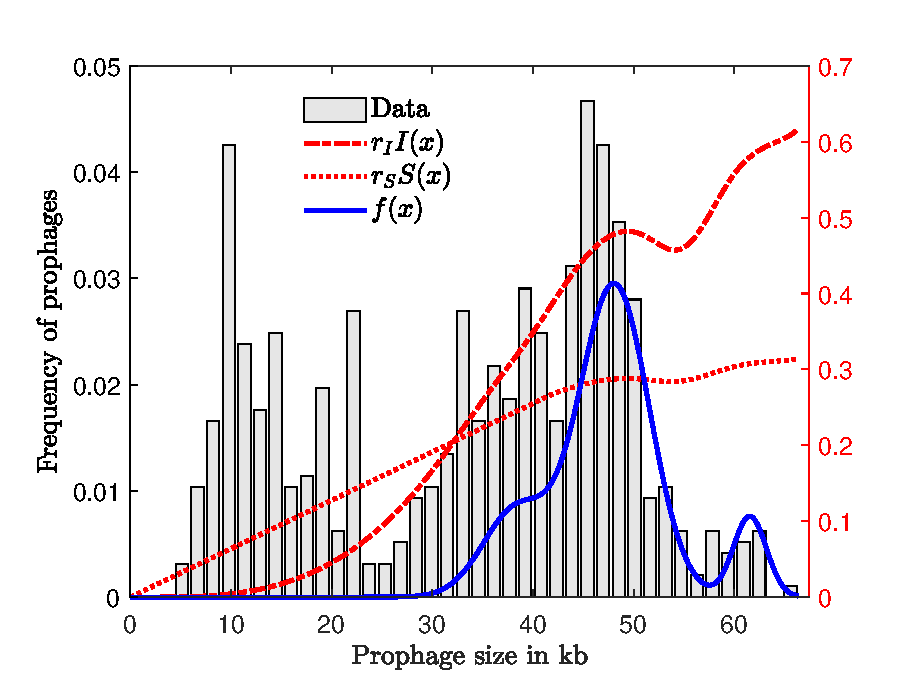
\includegraphics[scale=0.65]{combined1}
\caption[Components of the best-fit model prediction for Data Set 1.]{Components of the best-fit model prediction for Data Set 1 (histogram, left axis).  The distribution of autonomous temperate phages ($f(x)$, solid curve) is plotted along with the induction curve ($r_I I(x)$, dash-dotted, right axis) and the selection curve ($r_{S}S(x)$, dotted, right axis); induction and selection intersect near 30 kb.}
\label{fig:combine}
\end{figure}

An unexpected result of our analysis is that a process that preferentially adds prophages of shorter lengths to bacterial genomes (the process we describe as HGT in the model derivation) was not required to provide a fit to any of the three data sets.  For Data Set 1, HGT was included in the second-best fit, but the overall rate of HGT was extremely small relative to other rates in the model.  These results of course do not preclude a role for HGT in the maintenance of prophages in bacterial genomes, but indicate that HGT is not required to explain the empirical data currently available.  As mentioned previously, it seems likely that transduction may be the most important HGT process for prophages, and transduction rates are inferred to be low relative to other modes of HGT \citep{volkova_modeling_2014}.

Our findings suggest that a minimum of two to three prophage genes are required to enable prophage excision from the bacterial chromosome. The excision of phage $\lambda$, for example, requires at least two enzymes, an integrase and  exonuclease, which are produced from a single transcript encoding the $xis$ and $nit$ genes \citep{weitz_quantitative_2017}. We would of course expect wide variability in these steps across phage-host systems.  For example, phage Mu replicates first and then excises from the host chromosome \citep{10.2307/66893}, and would presumably require further intact genes for excision.

The relation between prophage and their bacterial hosts may either be parasitic or mutualistic depending on the balance between the cost the bacterial host incurs due to the integration of foreign DNA into its genome, and benefits conferred by the foreign DNA to the bacterial host \citep{shapiro_evolution_2018}. The biggest cost is incurred by induction, although due to the compactness of bacterial genomes, small insertions of foreign DNA may result in significant energy costs as well \citep{koonin_evolution_2009}.  Our results predict a tipping point between parasitism and mutualism, the point at which $r_I I(x) = r_S S(x)$.  Shorter prophage sequences are unlikely to maintain all the genes required for induction, and our model predicts that they persist at high frequencies in host genomes because of the selective benefits they still confer.  Thus the peak on the left of the bimodal prophage distributions may correspond to predominantly mutualistic prophage, consistent with high levels of purifying selection inferred for prophage genes using comparative genomics \citep{bobay_pervasive_2014}.  Metagenomic data, that is, prophage distributions obtained from environmental samples of bacterial populations, could help clarify the role of positive selection in maintaining prophage sequences.

Although an active body of research addresses the comparison and refinement of algorithms for prophage identification \citep{song_prophage_2019, sousa_phageweb_2018}, short prophage remnants can be difficult to detect and are likely underrepresented in the available data.  For example, prophage remnants with sequence similarity to short mobile genetic elements were excluded from Data Set 1 \citep{bobay_pervasive_2014}, and a minimum of six phage-like genes are required to identify phage gene clusters in the PHAST search tool \citep{zhou_phast:_2011}. 
Most algorithms to date rely on homology-based techniques to identify prophages, making it difficult to detect prophages that are not similar to known phages (but see \cite{akhter_phispy:_2012}), and making the identification of shorter sequences more challenging.   
This detection bias likely shifts the position of the lower peak in bimodal prophage distributions -- the true peak in the data might occur at even shorter prophage lengths -- but would not affect our conclusions regarding the underlying mechanisms in play.

We note that for one of the three data sets in this analysis, the best fit to the data was obtained using 14 of 15 possible parameters, that is, the best fit supported a relatively complex model.  This implies that as richer data sets become available, further features could, and should, be added to the model to better describe the prophage distribution.  As mentioned previously, two assumptions that could clearly be relaxed are that all phage genomes, irrespective of their length, offer the same average selective benefit to their host, and require the same number of genes for induction.  In reality, longer active phages presumably have the capacity to encode further beneficial functions and more complex excision mechanisms.  Another assumption, inherent in our approach, is that degraded prophage have lost the genes required for induction, or the genes conferring benefit to the host, in proportion to their total gene loss.  Thus the selection or induction rates depend only on prophage length. A more nuanced (but less tractable) approach will be to follow the loss and enrichment of specific classes of genes in degraded prophage sequences.

\section*{Acknowledgements}
The authors are indebted to Alita Burmeister for several insightful comments that strengthened the work.  The Natural Sciences and Engineering Research Council of Canada is gratefully acknowledged for funding.
 
\addcontentsline{toc}{chapter}{Bibliography}
\bibliographystyle{abbrv}
\bibliography{refrence}
% \begin{appendices}
% \chapter{Results from model selection and data fitting}\label{a2}
% The AIC value is the measure of loss of information for the model under consideration and is an ordinal number, used for ranking models. The lowest AIC value corresponds to the best fit.  If the number of data points are small enough compared to the number of parameters then the AIC value is not penalized enough. To remedy this problem a second order Akaike Information criteria, the corrected Akaike Information Criteria (AICc), is defined. The corrected  Akaike Information Criteria (AICc) is given as \citep{burnham_model_2003}:
% \begin{eqnarray}\label{aicc}
% AIC_c=AIC + \frac{2k(k+1)}{n-(k+1)}.
% \end{eqnarray}
% As the number of data points becomes large enough, AICc values converge to AIC values and either of these criteria can be used to determine the best fit model amongst the candidate models \citep{burnham_model_2003}. In the tables to follow, we provide both AIC and AICc values, and compute relative probabilities using the AICc values.
%   \section{Data Set 1}
% \begin{table}[H]
% \centering
% \begin{tabular}{ p{1cm}p{2cm}p{2cm}p{2cm}p{2cm}p{3cm}  }
% \hline
% \# & Parameters & AIC & AICc& Log-likelihood & Relative probability (AICc) \\
% \hline
% 1&                        15&          4884.1734&          4884.9642&         -2427.0867&         0.3719\\
% 2&                        14&          4882.2952&          4882.9860&         -2427.1476&         1\\
% 3&                        12&          4893.5207&          4894.0322&         -2434.7603&       0.0039\\
% 4&                        11&          4894.7613&          4895.1920&         -2436.3807&       0.0022\\
% 5&                         9&          4908.5087&          4908.8014&         -2445.2544&      2.4788e-06\\
% 6&                         8&          4906.2759&          4906.5097&         -2445.1379&      7.7964e-06\\
% 7&                         6&          5044.8136&          5044.9499&         -2515.9068&      6.7604e-36\\
% 8&                         6&          5069.6683&          5069.8042&         -2528.8341&      2.7098e-41\\
% 9&                         4&          5063.9143&          5063.9788&         -2527.9571&      4.9878e-40\\
% \hline
% \end{tabular}
% \caption[Number of parameters, AIC, AICc values, log-likelihood and the corresponding relative probabilities for Data Set 1.]{Number of parameters, AIC, AICc values, log-likelihood and the corresponding relative probabilities for Data Set 1 \citep{bobay_pervasive_2014}. The best fit model includes a mixed distribution to describe autonomous temperate phages ($g$=3), degradation, induction and selection. The second best fit model is the same model with HGT and has relative probability $0.3791$.}
% \label{table:bob}
% \end{table}
% \section{Data Set 2}
% \begin{table}[H]
% \centering
% \begin{tabular}{ p{1cm}p{2cm}p{2cm}p{2cm}p{2cm}p{2cm}  }
% \hline
% \# & Number of Parameters & AIC & AICc& Log-likelihood  & Relative probability \\
% \hline
% 1&                         15&          993.726&          998.583&         -480.863&       0.0016\\
% 2&                        14&          990.549&          994.797&         -480.275&        0.0108\\
% 3&                        12&          991.327&          994.492&         -482.663&         0.0126\\
% 4&                        11&           987.247&          989.937&         -481.624&         0.123\\
% 5&                         9&          987.197&          989.062&          -483.599&         0.191\\
% 6&                         8&          984.237&          985.749&         -483.119&          1\\
% 7&                         6&          1006.929&          1007.855&         -496.464&      1.585e-05\\
% 8&                         6&          1012.234&          1013.159&         -499.117&       1.117e-06\\
% 9&                         4&          1004.729&          1005.216&         -497.364&      5.927e-05\\
% \hline
% \end{tabular}
% \caption[Number of parameters, AIC, AICc values and the corresponding relative probabilities for Data Set 2.]{Number of parameters, AIC, AICc values and the corresponding relative probabilities for Data Set 2 \citep{crispim_screening_2018}. The best fit model includes degradation, induction and selection as well as one Gaussian distribution to describe autonomous temperate phages ($g$=1).}
% \label{table:desu}
% \end{table}
% \section{Data Set 3}
% \begin{table}[H]
% \centering
% \begin{tabular}{ p{1cm}p{2cm}p{2cm}p{2cm}p{2cm}p{2cm}  }
% \hline
% \# & Number of Parameters & AIC & AICc& Log-likelihood  & Relative probability \\
% \hline

%  1&                       15&          5671.819&          5672.579&         -2819.909&        0.0318\\
%  2&                       14&          5669.819&          5670.489&         -2819.909&        0.0904\\
%  3&                       12&          5670.179&          5670.685&         -2822.089&        0.0819\\
%  4&                       11&          5667.438&          5667.872&         -2821.719&          0.3347\\
%  5&                        9&          5667.461&          5667.766&         -2823.731&         0.3528\\
%  6&                        8&          5665.434&          5665.683&         -2823.717&         1\\
%  7&                        6&          5731.084&          5731.239&         -2858.542&      5.8167e-15\\
%  8&                        6&          5757.726&          5757.880&         -2871.863&      9.5404e-21\\
%  9&                        4&          5753.680&          5753.762&         -2871.840&      7.4776e-20\\
% \hline
% \end{tabular}
% \caption[Number of parameters, AIC, AICc values and the corresponding relative probabilities for Data Set 3.]{Number of parameters, AIC, AICc values and the corresponding relative probabilities for Data Set 3 \citep{leplae_aclame:_2010}. The best fit model includes degradation, induction and selection as well as one Gaussian distribution to describe autonomous temperate phages ($g$=1). }
% \label{table:aclame}
% \end{table}
% \newpage
% \chapter{Sensitivity Analysis}
% \section{Sensitivity to the smallest autonomous phage length.}\label{bob30}
% We tested fitting model (\ref{pde}) to Data Set 1, but assuming that the smallest autonomous phage to infect \textit{E.~Coli} and \textit{S.~Enterica} has length $\theta$ = 30 kb, as suggested in \cite{bobay_pervasive_2014}. We compared these results to results obtained with $\theta$ = 20 kb, as described in Section 2.2 of the main text. Figure~\ref{fig:comp_PDF} demonstrates that our results are insensitive to the choice of this parameter. 
% \begin{figure}[t]
% \centering
% 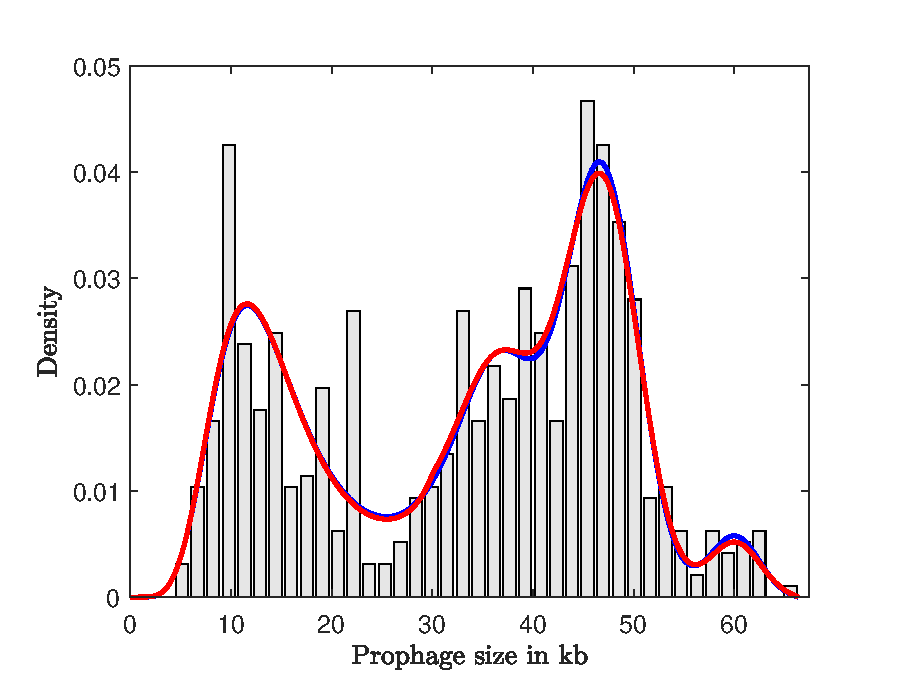
\includegraphics[scale=0.65]{comp_PDF.eps}
% \caption[Results of data fitting are not sensitive to the choice of the parameter $\theta$.]{Results of data fitting are not sensitive to the choice of the parameter $\theta$ representing the genome size of the smallest autonomous temperate phage in kb.  Best fits obtained to Data Set 1 (histogram) for $\theta$ = 20 (blue, solid) and $\theta$ = 30 (red, solid) are indistinguishable.}
% \label{fig:comp_PDF}
% \end{figure}
% \section{Rate parameters}
% We performed a bootstrap sensitivity analysis for all parameters of the model using Data Set 1.  In brief, we assumed that the best fit model for Data Set 1 represented the true distribution, and resampled this true distribution 335 times, each time creating a simulated data set of 624 observed prophage lengths.  We then subjected each of these data sets to the model fitting exercise described in Section 3 of the main text.  Table \ref{table:sens_p} shows the mean and standard deviations for the relative rate parameters of the model (each rate normalized by the induction rate, $r_I$), after the analysis of 335 simulated data sets.  These results indicate that the quantitative conclusions of our work are relatively insensitive to variations in data sampling; the coefficient of variation (standard deviation/mean) of the degradation rate is largest at 16\%.
% %\renewcommand{\baselinestretch}{1}
% \begin{center}
% \begin{table}[t]
% \centering
% \begin{tabular}{ p{1.6cm}p{5cm}p{2cm}p{2cm}p{2.1cm} }
% \hline
% Parameter & Description  & Mean & Standard deviation & Coefficient of Variation  \\
% \hline 
% \\
%  $\alpha $   & Relative rate of lysogeny &     0.2078&          0.0118 & 0.0569\\
%  $r_D$   & Relative rate of degradation &       0.0125&         0.0021 & 0.1644\\
%  $r_S$ &   Relative selection coefficient &    0.5012&     0.0483 & 0.0964\\
% % $r_I$ & Relative rate of induction & 1.0000 &  ---& --- \\
% % \\
%  \hline
% \end{tabular}
% \caption{Sensitivity analysis of rate parameters. }
% \label{table:sens_p}
% \end{table}
% \end{center}
% %\renewcommand{\baselinestretch}{2.0}

% \section{Influx of active phage, $f(x)$}

% In addition, this process produced 335 estimates of the influx distribution $f(x)$.  In Figure \ref{fig:sens_f}, we plot the mean of these functions at every value of $x$ (blue line), plus/minus one standard deviation (grey area).  The best fit $f(x)$ from Data Set 1 is also shown for comparison (red line).  These results indicate that the form of $f(x)$ is very tightly constrained by the data, a result that is perhaps not surprising given the large number of data points.

% \begin{figure}[t]\centering
% 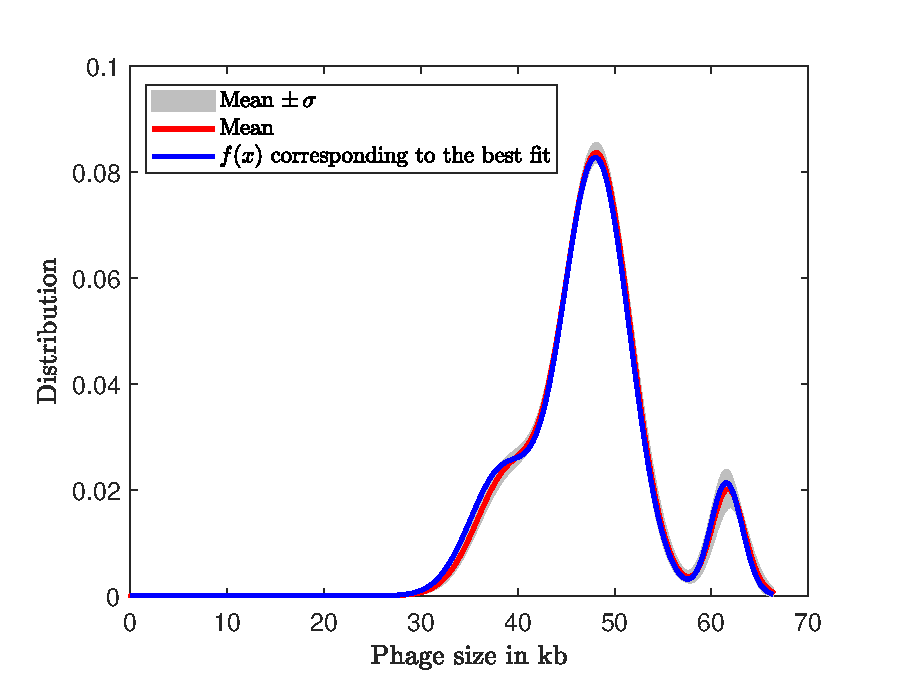
\includegraphics[scale=0.65]{f_sens.eps}
% \caption[Sensitivity analysis of the prophage influx function.]{Sensitivity analysis of the prophage influx function.  The mean (red) and standard deviation ($\sigma$) of best-fit $f(x)$ curves for all simulated data sets are shown, along with the best-fit $f(x)$ function from the true data (blue).  See text for details.}
% \label{fig:sens_f}
% \end{figure}

% \newpage
% \chapter{The influx distribution}

% As described in Section 2.2 of the main text, the function $f(x)$ gives the length distribution for prophages that are newly integrating into bacterial genomes.  Here, we note that this is neither the length distribution of active temperate phages, nor is it the length distribution of inducing phage.

% To clarify, suppose $A(x)$ is the length distribution of active temperate phages. Let $L(x)$ be the average lysogeny probability for a temperate phage of length $x$.  Since $A(x)$ consists of phages of different classes (lambdoid, mu-like, etc.), we expect that $L(x)$ is not constant in $x$.  In this case, the influx distribution  $f(x)$ is given by
% the product $f(x) = A(x)L(x)$.  Thus, unfortunately, we cannot use empirical data describing $A(x)$ to infer $f(x)$.

% Similarly, from the model at steady state, the product $P(x)I(x)$ gives the length distribution of excising prophage.  Suppose $R(x)$ gives the probability that a prophage of length $x$ retains the genes required for re-infection (genes involved in replication, packaging, and adsorption, for example).  If re-infection competent phage enter the lysogenic life cycle with probability $L(x)$, we could also express the influx distribution as $f(x) = P(x)I(x)R(x)L(x)$.  Again, we are unable to use $P(x)I(x)$ to directly infer $f(x)$.

% Despite these limitations, some qualitative features of $f(x)$ and $A(x)$ appear surprisingly robust.  Along with prophage sequences, the length distribution of 68 dsDNA temperate phages infecting enterobacteria are reported in \cite{bobay_pervasive_2014}.  While the weight of the peaks in this multimodal distribution vary, the number and position of the peaks is strikingly similar with our best fit estimate for $f(x)$ for Data Set 1, as shown in Table \ref{table:sens_f}.

% %\renewcommand{\baselinestretch}{1}
% \begin{table}[t]
% \centering
% \begin{tabular}{ p{6cm}p{2cm}p{3cm} }
% \hline
% Feature & Empirical Data & Model Prediction  \\
% \hline
% \\
%  Number of main peaks&     3&          3\\
%   Position of first peak&        $\approx 40$ kb&          $\approx38$ kb\\
%  Position of second peak &    $\approx 45$ kb &          $\approx 48$ kb\\

%  Position of third peak&       $\approx 59$ kb&      $\approx 61$ kb\\
%  \\
%  \hline
% \end{tabular}
% \caption[Comparison of the main features of empirical data describing the length distribution of autonomous dsDNA phages and the best-fit model predictions for the phage influx distribution.]{Comparison of the main features of empirical data describing the length distribution of autonomous dsDNA phages \citep{bobay_pervasive_2014}, and the best-fit model predictions for the phage influx distribution, $f(x)$. }
% \label{table:sens_f}
% \end{table}
% Similarly, we find that $I(x)P(x)$ yields a surprisingly good approximation for $f(x)$, as illustrated in Figure \ref{fig:IP}, again for Data Set 1.  This suggests that most prophage sequences that retain the genes for necessary for excision also retain the genes necessary for re-infection.
% \begin{figure}[t]\centering
% 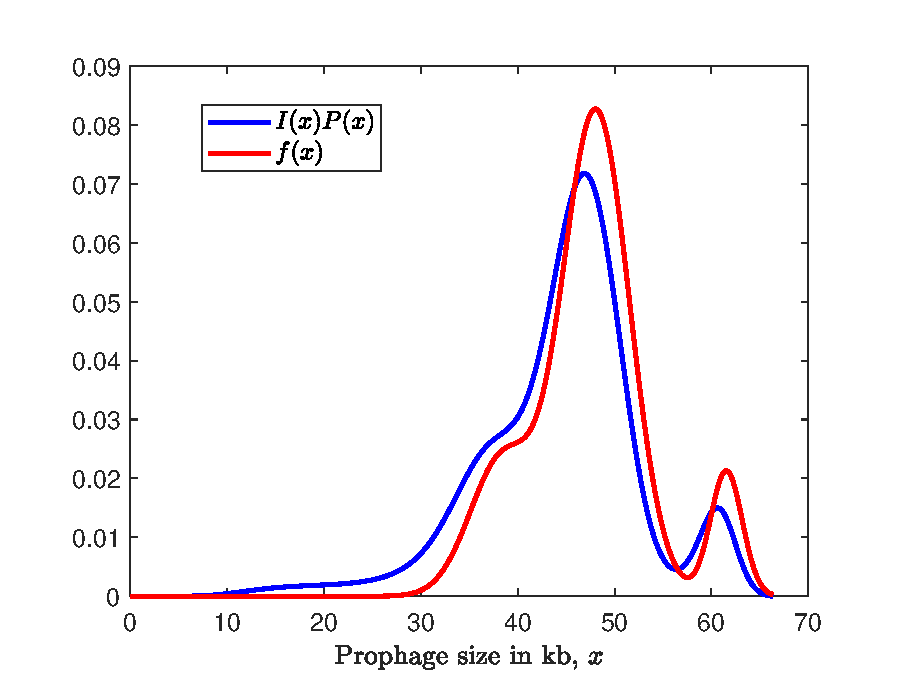
\includegraphics[scale=0.65]{IP.eps}
% \caption[Comparison of best-fit $f(x)$ with the product $P(x)I(x)$.]{Comparison of best-fit $f(x)$ with the product $P(x)I(x)$; results shown for Data Set 1.}
% \label{fig:IP}
% \end{figure}
% \end{appendices}
